\documentclass[a4paper, 11pt]{report}

% Venturer Camp 2023 Final Report & Evaluation preamble


% BASIC PAGE SETUP
\usepackage{geometry}
\geometry{
a4paper,
total={170mm,257mm},
left=20mm,
top=20mm,
}
\setlength\parindent{0pt} % get rid of the stupid indent

% set toc depth to only show chapters
\setcounter{tocdepth}{0}

% use section numbering for everything up too and including subsubsection
\setcounter{secnumdepth}{3}


% PACKAGES

\usepackage{tikz} % Required for drawing custom shapes
\usetikzlibrary{arrows, backgrounds, calc, fit, math, mindmap, positioning, shapes, shapes.geometric, tikzmark}

\usepackage{xcolor}

\usepackage{pgffor}

\usepackage{titlesec}
\usepackage[T1]{fontenc}
\usepackage[hidelinks]{hyperref}
\hypersetup{
pdftitle={Venturer Camp 2023 Final Report \& Evaluation},
pdfauthor={Thomas Boxall},
}

\usepackage{pgf-pie}

\usepackage{ragged2e}
\usepackage{float}
\usepackage{multicol}
\usepackage{multirow}
\usepackage{longtable}

\usepackage{appendix}
\usepackage{pdfpages}


\renewcommand{\arraystretch}{1.6} % make cells vertically bigger
\usepackage{colortbl}

% Headers and Footers

\usepackage{fancyhdr}
\pagestyle{fancy}
\fancyhf{}
\fancyhead[L]{Final Report \& Evaluation}
\fancyhead[R]{Venturer Camp 2023}
\fancyfoot[L]{\leftmark}
\fancyfoot[C]{}
\fancyfoot[R]{\thepage}
\renewcommand{\footrulewidth}{0.4pt}
\addtolength{\topmargin}{-1.59999pt}
\setlength{\headheight}{13.59999pt}

\raggedbottom
% Venturer Camp 2023 Final Report & Evaluation Preamble (Titles)

\newcommand{\drawhexagon}[5]{
    % #1 - text
    % #2 - position
    % #3 - size
    % #4 - rotation
    % #5 - options
    \node[rounded corners, inner sep=0, ultra thick, regular polygon, regular polygon sides=6, minimum size=#3, rotate=#4, #5] at (#2) {#1}
}

\newcommand{\drawtext}[5]{
    % #1 - text
    % #2 - position
    % #3 - height
    % #4 - rotation
    % #5 - options
    \node[left, bg, rounded corners, minimum width=\paperwidth, minimum height=#3, text width=\paperwidth, rotate=#4, #5] at (#2){#1}
}

\definecolor{accent}{HTML}{6d8f41}
\colorlet{fg}{black}
\colorlet{fgalt}{darkgray}
\colorlet{fgacc}{black}
\colorlet{bg}{white}
\colorlet{bgalt}{lightgray}
\colorlet{bgacc}{orange}
\colorlet{border}{black}
\colorlet{borderalt}{darkgray}
\colorlet{borderacc}{orange}


\titleformat{\chapter}[hang]{\Huge\bfseries}{\textcolor{accent}{\thechapter\hspace{0.75em}}\textcolor{accent}{|}\hspace{0.75em}}{0pt}{\Huge\bfseries}
\titleformat{\section}[hang]{\LARGE\bfseries}{\textcolor{accent}{\thesection\hspace{10pt}}\textcolor{accent}{}\hspace{0pt}}{0pt}{\LARGE\bfseries}
\titleformat{\subsection}[hang]{\Large\bfseries}{\textcolor{accent}{\thesubsection\hspace{10pt}}\textcolor{accent}{}\hspace{0pt}}{0pt}{\Large\bfseries}
\titleformat{\subsubsection}[hang]{\large\bfseries}{\textcolor{accent}{\thesubsubsection\hspace{10pt}}\textcolor{accent}{}\hspace{0pt}}{0pt}{\large\bfseries}

\titlespacing*{\chapter}{0pt}{0em}{2em}

\newcommand{\partTitlePage}{%
  \begin{tikzpicture}[remember picture,overlay]

    \pgfdeclarelayer{bg}    % declare background layer
    \pgfdeclarelayer{fg}    % declare background layer
    \pgfsetlayers{bg,main,fg}  % set the order of the layers (main is the standard layer)


    \fill[bg] (current page.south west) rectangle (current page.north east);


    \foreach \i in {0.5,...,20} {\drawhexagon{}{$(current page.north west)+(2.5,0)$}{\i cm}{0}{accent!60,draw};}


    \foreach \i in {21,...,2} {\drawhexagon{}{$(current page.south east)+(-0.2,-0.45)$}{\i cm}{0}{accent!85,draw};}


    \begin{pgfonlayer}{fg}
    \drawtext{\raggedleft \LARGE\partname{} \thepart}{$(current page.center)+(9.5, -5.5)$}{3cm}{0}{text=fg,align=right};
    \end{pgfonlayer}

    \end{tikzpicture}%
}

% Customize the part page
\usepackage{titlesec}
\titleformat{\part}[display]
  {\Huge\bfseries\filcenter}
  {\partname{}\thepart}
  {0pt}
  {\partTitlePage\Huge\bfseries}


% redefine \chapter so it uses pagestyle=fancy
\makeatletter
\renewcommand\chapter{\if@openright\cleardoublepage\else\clearpage\fi
\thispagestyle{fancy}%
\global\@topnum\z@
\@afterindentfalse
\secdef\@chapter\@schapter}
\makeatother


\newcommand{\makeDocumentTitle}{%
\begin{titlepage}
    % \pagestyle{empty}
    % \newgeometry{left=0cm,top=0cm,right=0cm,bottom=0cm}

    \begin{tikzpicture}[remember picture,overlay]

    %%%%%%%%%%%%%%%%%%%% Layers %%%%%%%%%%%%%%%%%%%%%%%%
    \pgfdeclarelayer{bg}    % declare background layer
    \pgfdeclarelayer{fg}    % declare background layer
    \pgfsetlayers{bg,main,fg}  % set the order of the layers (main is the standard layer)

    %%%%%%%%%%%%%%%%%%%% Background %%%%%%%%%%%%%%%%%%%%%%%%
    \fill[bg] (current page.south west) rectangle (current page.north east);

    %%%%%%%%%%%%%%%%%%%% Background Polygon %%%%%%%%%%%%%%%%%%%%

    % top left
    \foreach \i in {0.5,...,20} {\drawhexagon{}{$(current page.north west)+(2.5,0)$}{\i cm}{0}{accent!60,draw};}

    % bottom left
    \foreach \i in {2.5,...,22} {\drawhexagon{}{$(current page.west)+(2.5,-5)$}{\i cm}{0}{accent!60,draw};}

    % center right
    \foreach \i in {0.5,...,22} {\drawhexagon{}{$(current page.north east)+(0,-9.5)$}{\i cm}{0}{accent!90,draw};}

    % bottom right
    \foreach \i in {21,...,2} {\drawhexagon{}{$(current page.south east)+(-0.2,-0.45)$}{\i cm}{0}{accent!85,draw};}

    %%%%%%%%%%%%%%%%%%%% Title + Subtitle %%%%%%%%%%%%%%%%%%%%
    \drawtext{\Huge{\textbf{Final Report \& Evaluation}}\\\Large\textsc{Venturer Camp 2023}}{$(current page.center)+(3.2,-3.2)$}{3cm}{-60}{text=fg,align=right};

    %%%%%%%%%%%%%%%%%%%% Author Name %%%%%%%%%%%%%%%%%%%%
    \begin{pgfonlayer}{fg}
    \drawtext{\Large\textsc{Woodcraft Folk}\\\Large\textsc{January 2023}}{$(current page.east)+(-0.5,-5.2)$}{2cm}{0}{text=fg,anchor=east,align=right};
    \end{pgfonlayer}

    %%%%%%%%%%%%%%%%%%%% Year %%%%%%%%%%%%%%%%%%%%
    \drawhexagon{\Large }{$(current page.west)+(2.5,-5)$}{2.5 cm}{0}{accent!60,draw,text=fg};

    \end{tikzpicture}
    \restoregeometry
\end{titlepage}
}

\usepackage{draftwatermark}
\SetWatermarkText{PROOF}
\SetWatermarkScale{1}

\begin{document}
\makeDocumentTitle

\tableofcontents


\part{Background \& Introduction} % 1
    \chapter{Coordinator's Introduction}

Welcome to the Venturer Camp 2023 Final Report \& Evaluation.\\

For the most part, this document has been co-authored by the entire Venturer Camp team, with the Coordinator and Woodcraft Folk Events Assistant producing the first draft. This section, however, has solely been written by me - Thomas Boxall, Camp Coordinator.\\

To coordinate such a big Woodcraft Event was a great privilege. I grew up as a young person in Woodcraft and after seeing the impact the Covid Pandemic has had on the young people of today, I'm honoured to be able to say that I've changed these young people's lives by giving them a space where they can be themselves, have fun, forget the pressures of the outside world and take part in workshops centred around Woodcraft Folk's values.\\

However, saying that the year which we made Venturer Camp happen in was an easy one - would be a lie. Just saying it was a difficult one would also be a lie. The year from August 2022 to August 2023 was probably one of the most challenging years I've had in my life, due to a number of things - my role in coordinating Venturer Camp being one of them. \\

Woodcraft Folk is really great at empowering young people to do things, look at me - I was 19 while coordinating this thing. However, it's not good at supporting them to do big scary things like this. To say the year I was coordinating Venturer Camp was tough on my mental health would be an understatement. I'm extremely grateful for those around me who were able to catch me when I fell, both in and out of Woodcraft. They were the reason I was able to coordinate the camp. You know who you are - thank you for that.\\

Saying this, Woodcraft is good at catching people. From speaking to teams while writing this evaluation - I wasn't the only one to struggle with the work. Many of the teams had more and more work piled onto them, or individual members within teams who initially agreed to take on a small role ended up being instrumental in the success of that team's work. Through all the ever-increasing workloads, teams pulled it off. They more than pulled it off, they did it so well that we didn't notice how well they did it - the ultimate sign of success when it all goes smoothly.\\

Why Woodcrafter's have to fall before they can be supported is something that we need to consider, as an organisation. We cannot leave this untouched if we want to be a sustainable organisation which supports its members to try new things.\\

Pulling an event like Venturer Camp 2023 together in 365 days is by no means an easy feat. The countless hours of dedication from Volunteers up and down the country were the reason 450 people were able to be together in a field for 7 days and mostly have a good time. The majority of the work required to pull this event together fell to a relatively small group of active volunteers. Whilst it may seem from the outside that we had a substantial number of volunteers involved in the project, many of these weren't able to commit to a large role leaving a small core team to do most of the work. Throughout this report, you'll hear about different teams' struggles with capacity and workload management. Every core team member should be commended for how well they managed, how well they coped with the ever-increasing workload and how well they rose to the challenge of pulling off a Venturer Camp in a year. Don't ever try and do it in a year again, it's a silly idea.\\

I'm extremely proud of everyone who had a part to play in the success of Venturer Camp, all those who contributed countless hours making meticulous spreadsheets; those who contacted suppliers and chased to get the cheapest and best meatballs they could; those who cleaned the toilets and showers; and especially those who turned up, tried something new and had fun. We wouldn't have done this without you - thank you for that.\\

I want to leave you to enjoy the rest of this evaluation with a quote: ``we do this because we love Woodcraft''.\\

Blue skies,\\

Thomas Boxall\\

Venturer Camp 2023 Coordinator\\
<thomas@woodcraft.org.uk>

    \chapter{Introduction to the Evaluation}
This Final Report \& Evaluation of Venturer Camp 2023 has been primarily compiled by Thomas Boxall, Venturer Camp 2023 Coordinator (Volunteer), and Millie Burgh, Woodcraft Folk Events Assistant (Staff).\\

Every effort has been made to ensure that this report is as accurate and representative of all teams as possible. However, there may be times where this was not possible. All data referenced throughout this evaluation is available on request. Please contact the Camp Coordinator should you have any questions or wish to seek clarification on anything.

\section{Methods Used}
Opinions and Thoughts from the wider coordination team were gathered through a series of interviews conducted by the Camp Coordinator and Events Assistant. \\

Feedback from participants was gathered during the event itself through a Workshop run on a village level. Not all villages submitted notes from their workshop, so participant evaluations may not be representative of all participants on site. \\

All Volunteers involved in the project were invited to complete a Google Forms questionnaire after camp where they could give feedback. As expected with a survey like this, not all volunteers have responded and those who have responded would fall at either end of the spectrum, either having lots of good things to say or lots of bad things. Conversations had with volunteers throughout the event have been included.
\begin{figure}[h]
    \centering
    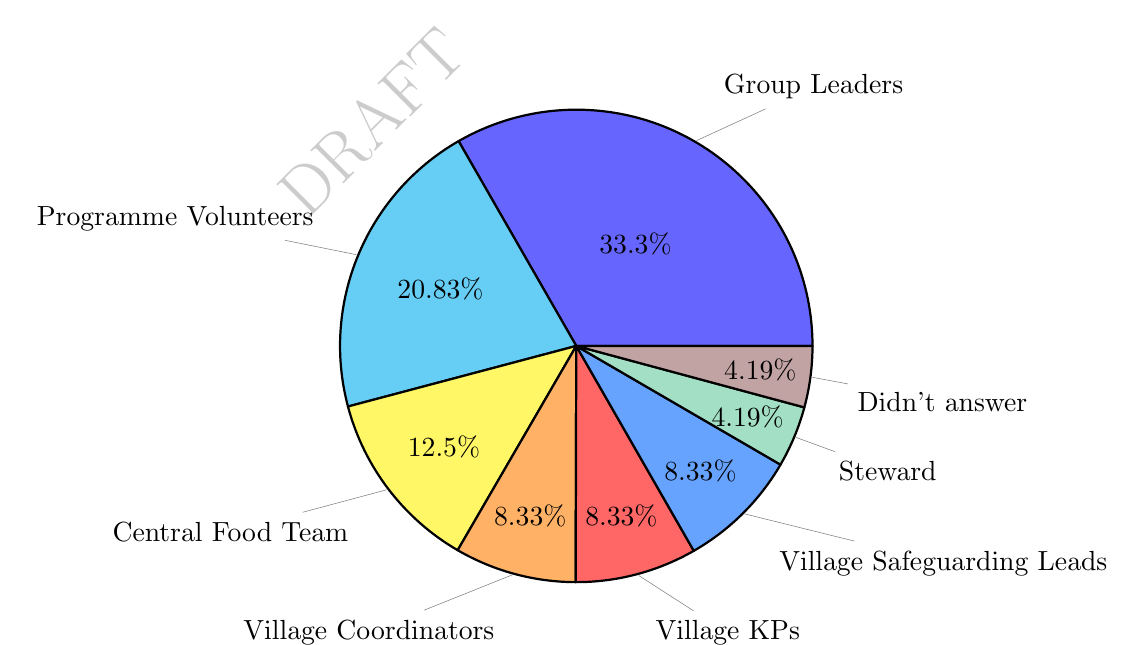
\begin{tikzpicture}
        \pie[text=pin]{33.3/Group Leaders,
        20.83/Programme Volunteers,
        12.5/Central Food Team,
        8.33/Village Coordinators,
        8.33/Village KPs,
        8.33/Village Safeguarding Leads,
        4.19/Steward,
        4.19/Didn't answer
        }
    \end{tikzpicture}
    \caption{Respondents to the Google Form Questionnaire}
    
\end{figure}

\section{Why Such A Long Evaluation?}
To put it simply, we should be evaluating our projects like this properly. Big camps are such a fundamental part of Woodcraft Folk's operations and with the organisation nearing its 100th birthday, you'd think we've got pretty good at getting lots of Woodcrafters in a field together having a good time. This is only mostly true, however.\\

This report aims to cover what we did, how we did it, and why we did it. As well as if it worked, how people found it and what we'd do differently in the future. \\

In all reality, there's going to be very few people who read the entirety of this document from cover to cover. However, people taking on roles at future large camps should be encouraged to read the sections relevant to them. 

\section{Photo Credits}
Photos have been used throughout this report, the captions include the initials of the photogropher, see below for names of those photographers:
\begin{description}
    \item[AB] Alex Baird
    \item[IC] Isabel Cleveland
    \item[RS] Ralph Sleigh
    \item[TB] Thomas Boxall
\end{description}

\section{Contact Information of Those Mentioned}
Due to this report being made available to the public on the internet, contact information of most people involved in this project has been redacted. The exceptions to this are Woodcraft Folk members of staff and the Camp Coordinator.\\

To obtain the contact information of anyone mentioned in the report - please contact Thomas Boxall, Camp Coordinator via \href{mailto:thomas@woodcraft.org.uk}{thomas@woodcraft.org.uk}

    \chapter{Introduction To The Project}
\section{Idea Conceptualisation}
Venturer Camp normally happens every 3 years, as a national camp for Venturers (the 13-15 year olds in Woodcraft Folk). 16 year olds are also normally allowed to come as participants if they haven't experienced a Venturer Camp before.\\

Typically a volunteer team provides infrastructure for the central area, a central menu, some central programme in the form of workshops in the daytime and some evening entertainment, and put groups in `villages' where they will eat, sleep and do clan. Group leaders bring their young people and organise their village including infrastructure, clans and activities.\\

For a long time Venturer Camp happened at Drum Hill Scout Campsite in Derbyshire, but in 2019 for the first time we held it at Biblins, Woodcraft Folk's own site in the Wye Valley. \\

There were two key things we wanted to do differently from past Venturer Camps this time round. Firstly, due to Common Ground being postponed 2 years because of COVID, this camp was to be 4 years after the Venturer Camp before opposed to the usual 3. For this reason, we expanded the participant age range to 17, to ensure as many young people as possible get to experience a Venturer Camp. \\

Another focus of this camp was volunteer support. Building on Common Ground, where for the first time there was a volunteer wellbeing role on the camp team, we wanted to ensure all volunteers (both central and village volunteers) were well supported on camp. We didn't manage to do as much as we wanted in this respect as we were only able to recruit one person for the volunteer support team who could support ahead of camp and on site, but the majority of the central team were able to get a day off with planning and support, which definitely hasn't been the norm in the past.

\section{Planning Timeline}
The decision was made in summer 2022 to hold a Venturer Camp the following August (we go into more detail why in the `What Dates' section). Because of this we only had a year to plan the camp when preparation usually starts around 2 years in advance. While most things don't happen until the final year, this extra year is pretty key when it comes to recruiting volunteers, building trust and care among the team and getting started with some key decisions and actions. Much of what could have been improved this camp came down to not having enough volunteers or volunteers not feeling confident/part of a team, which may not have been fully rectified by having an extra year but this almost certainly would have helped.\\

We have shown a Venturer Camp can be planned in a year, but not without either having a full team from early on or seriously overworking some members of the team. Therefore we would recommend always beginning plans 2 years in advance where possible.

\part{Event Decisions} % 2
    \chapter{Finding A Suitable Site}
For Venturer Camp 2023, the decision of what site to use was perhaps easier than in previous years. The accelerated timeline for the project meant that we would have had great difficulty finding a suitable site for Venturer Camp (thinking about infrastructure requirements on the site, transport links to the site, location in the country, etc).\\

Ultimately, we used Biblins Youth Campsite, which is owned by Forestry England and leased to Woodcraft Folk. Using a site which is managed by Woodcraft Folk, gives us greater flexibility and a level of quality assurance which would be unknown for other sites which we haven't worked with before.\\

From the feedback about the previous Venturer Camp's choice of site, also held at Biblins in 2019, you wouldn't have thought that we would use the site again. A large proportion of the campers commented that they were a very long distance from their village to the central area. These complaints were mostly from those camping on pitch 1 where they had to walk to Pitch 6 and 7 for the central programme. Since 2019, Biblins has undergone renovation works to relocate Camp Koodoo (its permanent camp) from Pitch 5 to adjacent to Pitch 1a. This resulted in us being able to centralise our central area onto pitches 4 and 5. We received little-to-no complaints about walking distance from villages to the central area, other than from those volunteers who would be in the central area up until meal times who would have to return to their village, collect food and then get straight back to the central area to finish programme delivery. This issue was quickly rectified, however, by the volunteers getting food delivered from their village to the central area. \\

For many months, the Coordination team had very little contact with the Biblins Staff Team; however, as camp approached, we had more contact with the team to gain information about the workings of the site, infrastructure on site and get copies of their policies and procedures which we would potentially need to implement while on site.\\

During the event itself, the Coordinator and Project Staff Team worked closely with the Biblins Staff Team, which enabled clear communication about issues and matters which arrose on site such as The Spill, access to the Bunkhouse Basement Storage and Adventurous activities, including a major change of plans to the Canoeing. \\

Having direct contact with the Biblins Staff Team proved invaluable and made the event considerably easier to organise.

    \chapter{Deciding on Dates}
\section{2023 v 2024}
As part of the project kick off, dates for the event had to be decided. However, before we could decide exactly which dates to host the camp on, we had to decide on a year first. This was a complex debate, with many people weighing in on the decision, ranging from Trustees to venturer group leaders to venturers themselves.\\

The ultimate decision was made that the camp should be hosted in 2023. We came to this decision based on the preference of Venturer Leaders and Venturers themselves to host the camp in 2023. This data was captured through a survey which ran for a few weeks in September 2022, the results of which can be seen in Table \ref*{tab:year-survey-results}

\begin{table}[h]
    \centering
    {\RaggedRight
    \begin{tabular}{p{0.2\textwidth} p{0.2\textwidth} p{0.2\textwidth} p{0.2\textwidth}}
    \textbf{} & \textbf{2023} & \textbf{No Preference} & \textbf{2024}\\
    \hline
    \hline
    Leaders & 56\% & 11\% & 33\% \\
    \hline
    Venturers & 67\% & 11\% & 22\% \\
    \hline
    \end{tabular}
    } % end of rr     
    \caption{Results of Year Survey}
    \label{tab:year-survey-results}
\end{table}

The survey also provided space where the respondents could share any thoughts, feelings, or suggestions. The responses to this varied were varied, some of the responses are shown below:
\begin{itemize}
    \item ``I think another national camp would not be supported. We need to have district summer camps to get young people back into camping. We struggled like lots of districts getting pioneers to common ground without a summer camp next year we will struggle to get children back into summer camps after the disruption of covid''
    \item ``Some venturers want a `proper camp before they are too old.' Adults want a break in 2024 before 100 camp''
    \item ``It would be good to have a date to be able to add to the calendar and to try and not book family holidays at the same time.''
    \item ``Personally, I think sooner is best as delaying by another year will inevitably mean some venturers won't get the chance to go. The venturers were mixed in responses, with a small majority favouring 2023 but others saying either or 2024. If it is next summer, please avoid clashing with the international camp in Finland (24-31 July 2023). Also, a question from our venturers is whether DFs who missed their chance to go to VCamp because of covid would be able to attend? Thanks''
    \item ``I have a venturer and a DF happy to help''
\end{itemize}

At the time of making the decision, we did not have a fully fleshed out team. There were significant gaps of knowledge and experience in the following teams:
\begin{itemize}
    \item Food
    \item Site Services \& Production
    \item Programme
    \item Communications
    \item Access \& Inclusion
    \item Event Administration (however we expected this role to be done by the Woodcraft Folk Events Assistant, so weren't worried about recruitment)
\end{itemize}
The lack of some of these teams presented a challenge for project initiation as once we had decided on 2023, they couldn't influence it and as such this deterred people from joining the team.\\ 

A volunteer close to the coordinator who supported him a lot said ``it's very dangerous when we organise the camp in a very short timeframe with a big dependence on one individual as it puts them in a vulnerable position and goes against our aims and principles. Empowering people to take on roles they've not done before is good but they need support in place. We need to ask questions about how they are supported.'' It was these questions around support networks which were answered when they were asked; when the coordinator was struggling, not pre-emptively. Pulling off a Venturer Camp in such a short amount of time, with such a limited capacity team. was not an easy thing to do (yes we did have a large number of people on it but many were limited in their capacity to be involved due to other commitments). Woodcraft Folk put too much pressure on the Camp Coordinator who was also juggling many other things, see introduction, which should never happen again.

\section{Which Dates In 2023}
The decision of what dates we wanted to host the camp on came down to four things:
\begin{enumerate}
    \item The dates which Biblins was available
    \item Festivals \& other attractive-to-young-people summer events
    \item School Term Dates (taking into account the early return of Scottish Schools)
    \item Finnish International Camp Dates
\end{enumerate}

At first, we chose the dates Monday 7 August to Monday 15 August. These dates were put to the Coordination team who decided that we would rather start and end on a weekend to reduce the amount of annual leave adult volunteers would have to take.\\

After some deliberation, we decided on Saturday 5 August to Saturday 12 August. These dates did't clash with any major festivals, were early enough that Scottish Young People would have a few days between camp finishing and their term dates starting, there were a few days between the Finland International Camp finishing and Venturer Camp starting, however the whole of the campsite was not available for all of these dates. There was a group booked onto pitch 1a for the night of Saturday 5 August. The decision was made that we wouldn't need that part of the site for the first night and so could press on with publishing the dates and working out the rest of the timeline.

\section{Group on Pitch 1a}
We took a gamble with the group on pitch 1a being a nice group who wouldn't mind 450 people descending onto the site. For the most part, the gamble paid off - the group were lovely and were interested in what we were doing. However, at first they weren't keen on the numbers of people who were camping to the West side of The Spill. We gave them a wide berth after they indicated this and had no further complaints or comments from them. 
    \chapter{Booking Timelines}
Once we had decided on dates for the camp, we could begin to work backwards designing timelines to suit. We settled on the public timeline shown in Table \ref{tab:booking-public-timeline}

\begin{table}[h]
    \centering
    {\RaggedRight
    \begin{tabular}{p{0.3\textwidth} p{0.5\textwidth}}
    \textbf{Date} & \textbf{Event}\\
    \hline
    \hline
    27 January 2023 & Bookings Open\\
    \hline
    12 April 2023 & Early Bird Booking Deadline\\
    \hline
    26 May 2023 & Final Booking Deadline\\
    \hline
    \end{tabular}
    } % end of rr     
    \caption{Public Booking Timeline}
    \label{tab:booking-public-timeline}
\end{table}

As we were designing the booking timeline, we made the decision to not close bookings. We believed that if we were to fully close bookings then we would be at risk of people turning up to camp who hadn't booked and would want to book on the door, or worse - they wouldn't tell the camp coordination team they had arrived which would complicate number based operations, such as food distribution or village size. We made a conscious decision to brand the 26 May 2023 deadline as the ``Final Booking Deadline'' in hope that we would deter people from booking late, and for the most part, we did.\\

We also had a second timeline, this was created and was published in the Payment Policy for Individuals and Groups, however it wasn't pushed onto people so they may not have known the late bookings were an option. One group reported that they treated the Early Bird Booking Deadline as their internal final deadline and another reported that they would accept bookings right up to the camp starting as long as the young person paid what they owed. 
\begin{table}[h]
    \centering
    {\RaggedRight
    \begin{tabular}{p{0.3\textwidth} p{0.5\textwidth}}
    \textbf{Date} & \textbf{Event}\\
    \hline
    \hline
    27 January 2023 & Bookings Open\\
    \hline
    12 April 2023 & Early Bird Booking Deadline\\
    \hline
    26 May 2023 & Final Booking Deadline\\
    \hline
    10 June 2023 & Booking Content Deadline\\
    & Refund Request Deadline (ad-hoc)\\
    \hline
    22 July 2023 & Late Booking Deadline\\
    \hline
    12 August 2023 & Very Late \& On-The-Door Booking Deadline\\
    \hline
    \end{tabular}
    } % end of rr     
    \caption{Internal Booking Timeline}
    \label{tab:booking-internal-timeline}
\end{table}

The refund deadline was added in an ad-hoc manner. This was due to the number of people wanting refunds for individuals coming up to the final booking deadline. The refund deadline was written into the payment policy and a second version was published on 24 May 2023.\\

Ultimately, not closing bookings proved valuable as a number of additional volunteers were recruited at DF camp to come and support the MEST-UP provision. These people paid the highest amount to come, the very late booking price, which supported us to hit our booking income target.

    \chapter{Who Do We Want To Come, Who Came?}

\section{Expanded Age Ranges}
Venturer Camps are traditionally held every three years. This cycle was disrupted by holding Common Ground International Camp in 2022, which was displaced from 2020 due to the Covid Pandemic. Not being able to hold a Venturer Camp in 2022, meant that there is one year's worth of Venturers who would have missed out on their Venturer Camp experience. For this reason, we decided to expand the age ranges of Venturer Camp 2023. The decision was made to include 16 and 17 year olds as Venturers. This would mean a small number of people who attended the 2019 camp as a participant would also be able to attend the 2023 camp as a participant.
\begin{figure}[h]
    \centering
    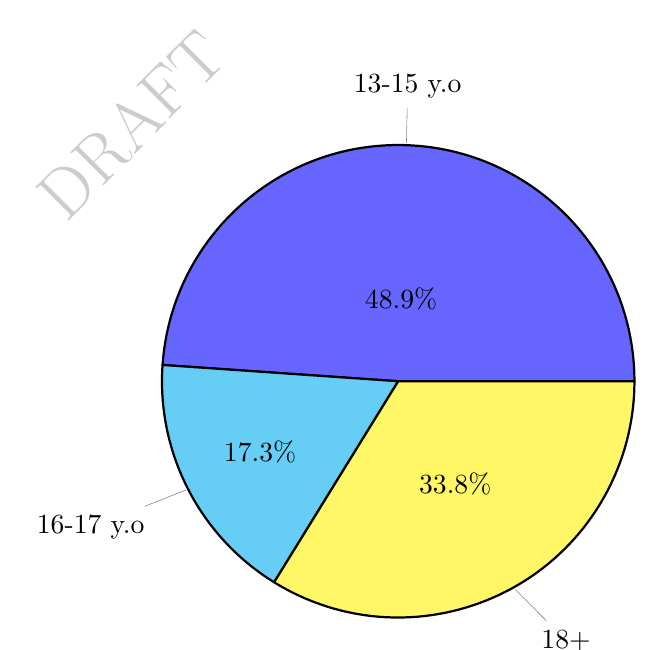
\begin{tikzpicture}
        \pie[text=pin]{48.9/13-15 y.o,
        17.3/16-17 y.o,
        33.8/18+
        }
    \end{tikzpicture}
    \caption{Booked attendees by age}
\end{figure}

By expanding the age ranges, we enabled more young people to participate in Venturer Camp 2023. We also enabled those 16 and 17 year olds who may never have experienced Woodcraft Folk outside their district or Common Ground, which was very structured, to have a looser structured Woodcraft Folk experience. The hope was that this would support them to transition to DFs, enabling them to grow their movement (the pandemic resulted in many DFs falling out of the movement). Figure \ref{fig:distribution-of-attendees} shows how some DFs were able to take on Volunteering roles as under-18 volunteers.
\begin{figure}[ht]
    \centering
    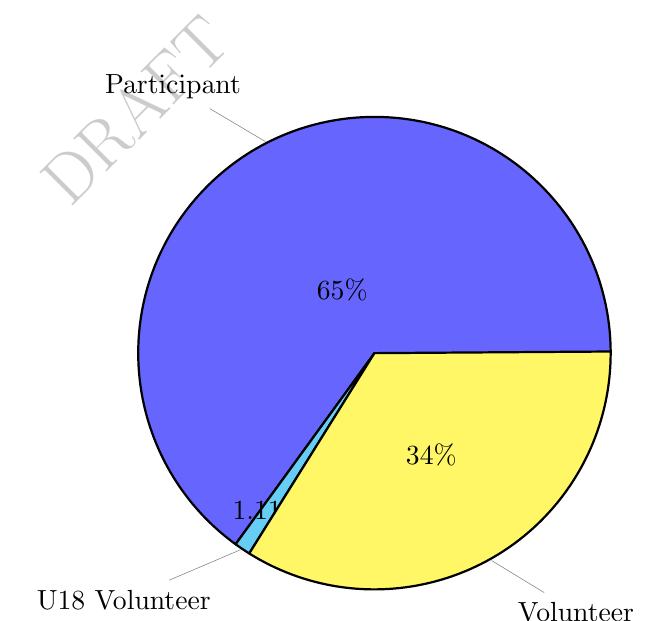
\begin{tikzpicture}
        \pie[text=pin]{65/Participant,
        1.11/U18 Volunteer,
        34/Volunteer
        }
    \end{tikzpicture}
    \label{fig:distribution-of-attendees}
    \caption{Distribution of Attendees}
\end{figure}

\section{International Delegations}
In Autumn 2022 we were also hoping that we would be able to support a number of international delegations to attend. We discussed a number of models through which we could facilitate this with a very small coordination team. The majority favoured being that a group or district would be responsible for all aspects of supporting an international delegation.\\

In Spring 2023, the general enquiries inbox was contacted about the possibility of hosting a group from an English Language school situated in Spain. However, due to the Woodcraft knowledge barrier and the implied expectation that we (the central coordination team) would be responsible for supporting this group to attend, the decision was made to decline this request. At this time, the coordination team was stretched very thinly, with many people taking on more than what they'd expected to be doing in the run up to the event.\\

We were, unfortunately, unable to host any international delegations at Venturer Camp 2023. 

\section{Centrally Organised Equipment}
During the conceptualisation of Venturer Camp 2023, we decided that to reduce burdens on Villages - we would centrally organise the equipment which was being assigned to Villages. This concept, what worked well and what didn't work about it will be explored in the Site Services \& Production Team's section - there are very mixed views about this!

    \chapter{Pricing}
After developing the booking timeline and deciding about the expanded age ranges, we were able to decide on pricing for the camp.\\

Woodcraft Folk is committed to working to reduce barriers towards Volunteering. One such barrier, Venturer Camp presented a perfect test ground for - is the financial commitment to come to a camp. This resulted in us having the following pricing structure.

\begin{table}[h]
    \centering
    {\RaggedRight
    \begin{tabular}{p{0.2\textwidth} p{0.2\textwidth} p{0.2\textwidth} p{0.3\textwidth}}
    \textbf{Before} & \textbf{Age Bracket} & \textbf{Whole Camp} & \textbf{1 night}\\
    \hline
    \hline
    \multirow{2}{*}{26 May 2023} & Under 18 & \pounds150 & \pounds21.50\\
    \cline{2-4}
    & 18 and over & \pounds50 & \pounds7.50\\
    \hline
    \multirow{2}{*}{22 July 2023} & Under 18 & \pounds225 & \pounds32.25\\
    \cline{2-4}
    & 18 and over & \pounds75 & \pounds11.25\\
    \hline
    \multirow{2}{*}{12 August 2023} & Under 18 & \pounds300 & \pounds43\\
    \cline{2-4}
    & 18 and over & \pounds100 & \pounds15\\
    \hline
    \end{tabular}
    } % end of rr     
    \caption{Pricing Structure based on 1-person figures}
\end{table}
We made the decision that all those attending the camp who are aged 18 and over would be attending as a volunteer, and as such we would recognise their contribution by charging them a third of the participant cost. 

\section{Under-18 Volunteer Priced Places}
Due to the enlarged age ranges for Venturer Camp 2023, we also wanted to ensure those who could technically come as participants had the opportunity to volunteer without paying the (higher) participant price.\\

This desire led to the creation of the Under 18 Volunteer Price Scheme whereby a young person aged 16 or 17 could apply for a volunteer priced place if they were at the camp primarily as a volunteer. The scheme required a few things of the young person before the price reduction could be allocated: 
\begin{enumerate}
    \item have begun the process of obtaining a Enhanced DBS (or membership of the PVG scheme if based in Scotland);
    \item be registered as a member of Woodcraft Folk and have paid their membership fee;
    \item have submitted references (this will normally have been done as part of becoming a member of Woodcraft Folk); and 
    \item have spoken to the relevant team leader about the role and a volunteer role description has been produced (this should be included with the application).
\end{enumerate}
This scheme was widely publicised, and despite this - we only had approximately 5 people take part in it. The roles they took on ranged from stewarding to centre coordinator to cafe \& special diets kitchen assistant.\\

There were a number of young people who had paid the participant price who attended to volunteer. These young people coordinated a centre as a group. They made the decision to pay the participant price as they also engaged in some other programme. For future events, it might be worth having an intermediary pricing point for those young people who are volunteering some of the time and also participating at other times. 

    \chapter{International Volunteers}
After Brexit, organisations in the UK are no longer eligible to participate in the European Solidarity Corps (ESC) programme run by the European Commission. Common Ground (2022 International Camp) was supported by a 15-strong team of ESC volunteers and as such, it was hoped that Venturer Camp 2023 would also be able to be supported by a number of international volunteers as those at Common Ground proved extremely valuable to the team.\\

Woodcraft Folk worked with a UK-based charity called Concordia to manage the recruitment of volunteers. A further evaluation of how this worked, what went well and what didn't work can be found in the Concordia chapter.

    \chapter{Venturer Committee's Involvement}
At the time of project kick-off for this event - there was no functioning Venturer Committee. This was due to the pandemic and the fact that all the current members had `aged-out'. This led to there being very little involvement in the planning process from Venturer aged people. It was an unfortunate loss to not have young people's voices on the planning committee. We had hoped to overcome this shortfall with a scheme called the \textit{Village People}

In September 2022, a meeting was held between key individuals where it was discussed about using Venturer Camp as a chance to re-form Venturer Committee. Due to a combination of factors, including lack of capacity in progressing with re-forming Venturer Committee, nothing happened with this until camp itself started.

On Camp, an individual planned and held Venturer Committee elections with the support of previous Facilitators. The elections held at the event were a great success and all roles on Venturer Committee were able to be filled. This individual also held other roles of responsibility on camp, and as such they had a very busy time. For future events, it would be recommended that an individual with no other commitments takes on the Venturer Committee Elections Facilitation role.

\section{Village People}
The Village People was a scheme designed to introduce the voice of the participants and the people who knew the participants the best into the planning of Venturer Camp 2023. In Autumn 2022, we invited all Venturer Leaders to apply to join the group. We then selected a representative sample, ensuring all types \& sizes of groups were represented.\\

The scheme unfortunately died out quite quickly due to extremely low response rates to opinion-gathering forms which went out. It would be lovely to see a scheme like this work at a future large Woodcraft Camp. 

\part{Event Administrations \& Communications} % 3
    \chapter{Bookings}
\section{Booking System}
After discussions between the Camp Coordinator and Woodcraft Folk Chief Executive where different booking system options were reviewed, it was agreed to use Ralph Sleigh's custom system which had been first used at Venturer Camp 2019, then Common Ground 2022. Ralph and the Camp Coordinator had initial conversations about what features the booking system would require as Ralph had started re-writing the booking system to use different, more cost effective, technology.\\

During Autumn 2022, the Food and Special Diets teams were consulted about what data they wished to collect from those booking in. As the focus on special diets was new to Woodcraft Camps, a larger amount of data was captured about each individual booked on. Through using the custom booking system, the implementation of this was exactly as we wished, while using an off-the-shelf system we may not have been able to collect and view this data in the same way.\\

During January 2023, the booking system was tested with the core team. These tests enabled the workflow of approving bookings, the mechanics of booking and ensuring that the wording used in the system was clear. Also during this period, the Booking Handbook was written.\\

The decision was made to require ``applications to book'' before enabling people to book. This decision was made mostly by the fact that Common Ground used this feature. In reflection, it was the right decision to use as it enabled us to ensure people booked in a way that was convenient to us. Rather than individuals booking, we had larger groups booking and we had the say to stop individuals if needed where there was already a group booking for their group. This also enabled us to ensure there were no bookings from people unknown to Woodcraft, but we either received no or very few requests of this nature.\\

Throughout the use of the booking system, a number of bugs and issues arose with it. Ralph responded quickly to all of these, deploying a fix usually within 12 hours of the issue being reported. Ralph was also able to implement features which improved the usability of the system, for example, messaging manager messages to the Coordination Team Discord server which prevented the need to use the emails the system also sent.\\

Overall, the use of a booking system which was developed ``In house'' gave us greater flexibility, greater options and overall a much easier experience than that of an off the shelf system. \\

The booking system allowed users to be able to be assigned backend access to view some or all of the data entered by users. To ensure volunteers who were being given this access had some basic understanding of GDPR, a Data Protection Declaration was created which all backend users of the booking system were expected to sign before being granted access. This worked and while Woodcraft Folk is not providing basic GDPR training for its volunteers, is something which should be repeated for future events. The transcript of the declaration can be found in the Appendix.\\

One thing that wasn't so great about Ralph's system is that it couldn't automatically match up who has / doesn't have membership. Or at least we thought it couldn't. When we discussed this at one point Ralph said there was something he could try to rectify this, which is definitely worth exploring for future events which use this system. 

\section{Bookings Administration}
After the bookings opened - Thomas and Millie processed most of the administration around bookings. This involved things such as: managing applications to book, reviewing bookings to locate any access needs.\\

Before bookings opened - there were conversations around how we want people to book. The decision was taken to try to get people to book as groups, with the general principle of one booking per group; with central adult volunteers booking separately.
This system worked, mostly. There was one case in particular where a region decided to come together and due to the disconnected nature of the young people attending - they took the decision for all the parents to book their children on. Unfortunately, they decided to start making their booking on the date of the early booking deadline. This led to the booking applications being accepted.\\

With having the booking deadlines at midnight, this meant that the responsibility of being on standby to approve the booking applications which come in after the members of staff had finished for the day fell to a volunteer, which for this event fell to the Camp Coordinator. For future events, the booking system needs to be able to specify the time of a booking deadline so that it can be set for a more sociable hour! \\

The booking system generates a unique booking reference for each booking. This then means that when the money is transferred to the Woodcraft Folk Bank Account, we should be able to match up the payment to the booking. This works reasonably well, so far as people used the references and we were able to match up payments. The difficulties experienced with this system came from the structures of the Woodcraft Folk Finance Administration Systems, see below for a more detailed analysis of this. 

\section{Early Booking Deadline}
A decision was taken that the incentive for booking by the early-bird deadline was to receive a free limited edition t-shirt. This decision, whilst good in theory, creates a large financial overhead - where each t-shirt costs more than the financial discount would have been. Once this fact was discovered, it was agreed that we would expect people to have booked and paid their deposit by the Early Bird Booking Deadline to receive a free t-shirt.\\

The communications around the requirements for payment before the t-shirts were given out was not the best due to a number of factors. Primarily, it was down to time pressures that all locations promoting the early bird deadline weren't updated to reflect the payment requirement. The requirement to pay was communicated through the Payment Policy and through social media content leading up to the deadline.\\

Unfortunately, some groups didn't receive the message about the payment requirements. These caused tensions where group leaders had promised their young people free t-shirts and there were no free t-shirts for them as they had not paid by the deadline. These tensions were rectified by selling the group leaders t-shirts `at cost', rather than at the standard camp rate. Whilst not a perfect solution, it was accepted. \\

For those who did pay deposits \& book in advance of the deadline: a Google Form was used to gather the size requirements, which influenced the numbers of garments in each size we ordered. \\

It would not be recommended to do a free t-shirt as the reward for Early Bird bookings in the future. This is due to the complex administration requirements, and the difficulties experienced with advertising the offer

\begin{figure}[ht]
    \centering
    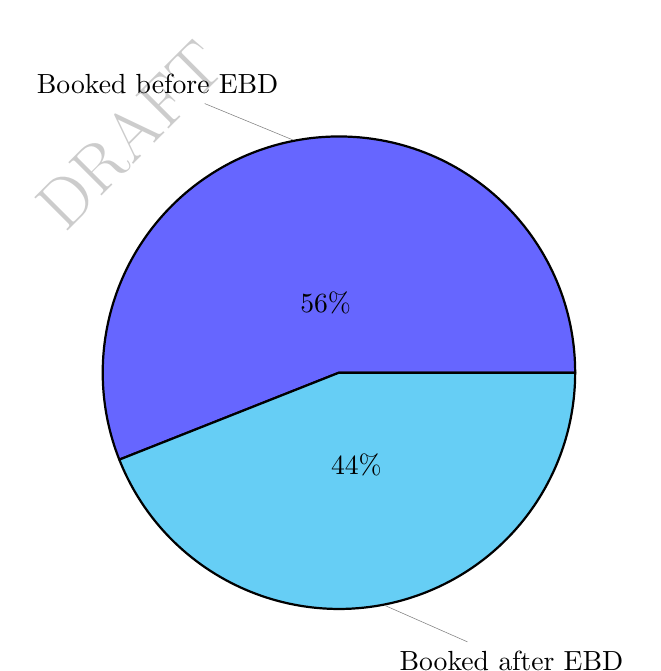
\begin{tikzpicture}
        \pie[text=pin]{56/Booked before EBD,
        44/Booked after EBD
        }
    \end{tikzpicture}
    \caption{Attendees booked before / after Early Bird Deadline (EBD)}
    
\end{figure}
    \chapter{Finance}
The finances for Venturer Camp 2023 were overseen by the Head of Resources at Woodcraft Folk with assistance and knowledge given from the Venturer Camp Treasurer and Coordinator. The decision to manage the finances like this came about from not having anyone in the treasurer post at the start of the project so the Coordinator and HoR began managing the finances themselves, then once a treasurer was appointed this felt like the simplest option. \\

The management of finances through the Woodcraft Folk systems had a number of benefits and drawbacks. The most notable benefit was that it was all dealt with for us (``us'' being the Core Team), with trained professionals managing the day to day running of the finance. The Treasurer was able to support by approving expenses and invoice payments as well as doing the first level of chasing for payments, later levels of chasing were done by the HoR.\\

One of the significant drawbacks of using the very established Woodcraft Folk finance system is that it is already set up very firmly. The Venturer Camp team's budget lines didn't match the central monitoring system, and this made our lives much more difficult when reviewing payments into and out of the account in order to monitor how much was being spent in each category. This was further exacerbated by the fact that the finance monitoring tools (a series of Google Sheets) were set up such that they required a great level of understanding to be able to read them. This resulted in large amounts of confusion amongst those people who had to read them and understand them. \\

Another significant drawback of using the Woodcraft Folk finance system was that quite often transactions were ``mis-coded'' within the system. This resulted in transactions erroneously appearing on the monitoring spreadsheet, or not appearing altogether - leading us to believe we hadn't spent as much as we in fact had. 

\section{Budget}
The first budget for Venturer Camp 2023 was drawn up by Woodcraft's Chief Executive using figures from Venturer Camp 2019 and Common Ground International Camp 2022 to influence expected expenditure for 2023. Throughout the project, minor alterations were made to the budget, mostly to reflect the change in expected income due to fundraising income being lower than initially expected.\\

Due to the above mentioned issues with income and expenditure coding within the Woodcraft Folk finance systems, and the fact that they do not line up with our budget lines - we do not have a final breakdown of expected vs actual for our budget.\\

Shown below is the Venturer Camp 2023 budget, compared to the Venturer Camp 2019 actual expenditure. 


    \chapter{Website \& Social Media}
\section{Website}
For historical Venturer Camps, the domain \texttt{venturercamp.org.uk} has been used. Having a separate domain provides a number of pros and cons, this was the cause of a lengthy discussion in Autumn 2022.\\

Ultimately, it was decided that the domain would be re-registered and a simple WordPress website would be created using a cheap shared hosting provider. Ralph Sleigh and Thomas Boxall met virtually to register the domain, choosing 123-reg as the domain registrar and Hostinger as the hosting provider. Ralph managed the domain registration and therefore configured the DNS records to ensure that the domain was linked correctly to the Woodcraft Folk Google Workspace.\\

Having our own website gave us the flexibility to publish whatever content we wanted and allowed us to configure the website exactly how we wanted to. The decision was taken to leave WordPress configuration as simple as possible, exclusively using off the shelf components as this would make our life as simple as possible! \\

The configuration of the website was for the most part left unchanged during the year which it was active for. Only two major changes were made: adding reCAPTCHA and changing the Home Page. \\
Adding reCAPTHCA to the contact form plugin we used (WP Forms) was done out of necessity. We were beginning to receive an unmanageable amount of spam to the WordPress comment queue and by adding ReCaptcha, we were able to reduce this to a more manageable amount. \\
Changing the homepage was done to be able to give out the most accurate information during camp - something which the initial homepage didn't allow for. \\

For the most part, the operation of the website was managed by Thomas, however a number of others also had access to edit and manage the content on the site. There had been plans to expand the number of editors on the website, to allow teams to publish their own news articles and content - however this never happened due to time limitations.

\section{Social Media}
After Venturer Camp 2019, there is an already-established Venturer Camp instagram account which we gained control of during October 2022. At the time, the Camp Coordinator was doing the comms role and as such began posting semi-regular content to the account. At the time, there was no plan used as there was little time to devise a plan.\\

While gaining access to social media accounts, Thomas also got into the Facebook account. Through this, he learnt that the 2019 camp used a profile, rather than a page which meant we wouldn't have had any statistical oversight from it. Thomas created a page and published a link to it across all social media platforms and we gained followers.\\

The Facebook and Instagram pages were both linked to the same Meta Business Account, which meant we had oversight and control over them both from one place.\\

Thomas took the decision to not use Twitter. A tweet was published informing followers of this fact and signposting them to where they could find out more.\\

Through October, November, December and January, Thomas took a lead on producing content for the social media platforms. Posts were sporadic and it was generally used as calls to action for volunteers rather than beginning to excite people for bookings to open. For future events, it would be massively beneficial to have a dedicated communications manager in the team whose responsibility it is to deal with pushing content to social media.\\

As pressures on the coordinator ramped up in different aspects of the camp, Thomas handed over the managing of the social media to the Events Assistant who managed the social media until late spring / early summer where Alex Baird, national Communications Volunteer,  took over the managing of the social media alongside Woodcraft Folk's Communications Manager. \\

The use of social media for an event like this has many different purposes, ranging from telling people bookings are open, raising people's excitement about the event and giving them all the critical information.\\

There were times that we were unable to create and push content out due to not having capacity. This was unfortunate as the event is catering for those who probably spend the highest amount of time out of any age group on social media.\\

Without the role of communications being filled on the team - we were in a situation where social media often fell to an afterthought. Whilst not ideal, we managed like this. There were enough people who had access to the social media accounts that something could be pushed out when absolutely necessary. For future events, having a dedicated communications team (for larger events) or person (for smaller events) is imperative. It is not something which should fall to the Coordinator to do. The coordination team should also have the space to share content through the social media when needed, another thing which we were unable to do due to the size of our team.

    \chapter{Written Communications}
\section{Mass Emails}
Throughout the coordination of an event like this, communication with the membership is a vital process. Within Woodcraft Folk - the main way in which this is done is through mass emails pushed out through Constant Contact (mass mailing platform).\\

No one on the Venturer Camp team had direct access to Constant Contact, this caused a number of problems as we were unable to send the mass emails ourselves. Whilst understandable from a GDPR standpoint, it caused some difficulties. The main difficulty was the inability to send an email on-the-fly. Emails would have to be booked in with the member of staff sending the email at least a week in advance of needing to send them with the content deadline often at least multiple days before the target email send date - to give the staff time to schedule the email to be sent. There were a number of times where these tight deadlines meant that the emails didn't contain all the information in them that was originally intended due to not having enough time to write them. \\

Towards the end of the project, when time pressures were higher, Gmail's Multi Send Mode was utilised as this meant that emails could be sent to multiple recipients without using BCC (as this often results in emails going directly to people's spam box) while maintaining GDPR compliance. This proved extremely effective as the Coordinator had control over exactly when emails were sent and the content of them therefore reducing the dependence on others to send emails therefore reducing the lead time to send a mass email.\\

Another issue encountered using Constant Contact was the mailing list inconsistencies. Initially, we were using a ``All Venturer Group Leads'' list which had been pulled from Groop in the Autumn of 2022 however towards the end of the project, it was more relevant to email just the booking contacts. This data was only accessible within the booking system which therefore meant, a new mailing list would have to be created each time a mass email was to be sent within Constant Contact to ensure that any new booking contacts or additional booking contacts were included. Once the final booking deadline had passed, this was less of an issue however it still presented edge-case challenges where extra individuals would book on and we would then need to ensure they too received the mass emails.\\

As we didn't have capacity to, we didn't think about tailoring emails to the two different groups of people who booked on: group bookings and individual bookings. There was quite often confusion amongst the individual booking contacts where their entire contact with Woodcraft before had been as a parent of a child attending a weekly group night. This added some additional administrative burden to respond to the individuals when they questioned what the email meant to them. In the future - it may be useful to tailor the mass-emails to the two groups.

\section{Big Month Updates}
Towards the later months in the project, we began to push out `Big Month Updates'. These were one-stop-shop updates which contained all the relevant content either for the upcoming month or about the month-just-gone. It was unfortunate that these updates were only started towards the end of the project as it was felt that they were useful.\\

A newsletter-kind of update proved useful to the coordination team as it was a regular chance to push updates to the wider movement. Shorter updates would still need to be pushed during the times between the larger updates as sometimes there were news items too critical to wait. \\

For future large Woodcraft camps, it would be suggested to review and look to keep going with larger newsletter style emails \& blog posts on the website. Through publishing to the website, you also make the content available to those not in direct receipt of the email. It would also be advisable to share the highlights through social media, ensuring you reach as many people as possible.

\section{Information Pack}
Another staple within Woodcraft Folk camps are the Info Packs. For Venturer Camp 2023, we produced 3 (v0, v1 and v2). \\

The info packs were timed to be released at strategic points in the academic calendar, providing group leaders the information they needed at the right time. It was felt that less questions came through around topics covered in the info packs than would be expected, suggesting that leaders found them a useful resource.\\

Info Packs were co-authored by the entire Venturer Camp team, with the Coordinator and Events Assistant taking a lead. Once the content was complete, the coordinator typeset the packs using \LaTeX. The proof copies of the documents were then shared to the team for further contributions / comments, and once amended - the document would be published to the website. 

\subsection{Info Pack v0}
Info Pack v0 was published in December 2022 and aimed to provide a single location where the initial information about the event could be found. The document included:
\begin{itemize}
    \item An introduction from Thomas \& introductions to the different teams
    \item Information around the bookings process
    \item Information surrounding the cost of camp, suggestions for local group fundraising \& the access fund
    \item How to get involved
    \item Early information around food at camp, focusing on the differences to previous camps
    \item Information on the Sustainability of Venturer Camp 2023 \& its environmental impact
    \item The dates for on-site pre-camp
\end{itemize}

\subsection{Info Pack v1}
Info Pack v1 was published in early May 2023. There had been plans to release a few weeks earlier however due to delays in some content, the publication of the pack was delayed. \\

Info Pack v1 contained much more information about the event, still with some unclear details however. Much of the pack was dedicated to logistics surrounding equipment, communications, programme and food at the event. The table of contents included:
\begin{itemize}
    \item Pre-Camp details, both virtual and on-site
    \item Travel to site logistics
    \item Communications during the event, including emergency contact details
    \item Equipment
    \item Food
    \item Programme
    \item Introduction to the International Volunteers
    \item Decarbonisation
    \item Volunteer Wellbeing
    \item Safeguarding \& Risk Management
    \item Site Safety
\end{itemize}

\subsection{Info Pack v2}
Info Pack v2 was published in late June. This was the last major update group leaders got before the Village Handbook was released in July. the table of contents included:
\begin{itemize}
    \item Repeat of much of the info pack v2 content, with some details further fleshed out
    \item Site Layout
    \item Village composition
    \item Further detail on programme offerings
    \item Greater details on Safeguarding \& Risk Management
    \item Price list for the Cafe and Merch stand
    \item  Remaining roles to be filled
\end{itemize}

\section{Village Handbook}
For Venturer Camp 2023, we wanted to go back to the historical ways of doing things - publishing the Village Handbook well in advance of the camp, ensuring those who needed it had the information, before they got to site. This methodology worked, and while there were a few minor amendments made on site - the main village handbook document was published two weeks before the start of camp.
\subsection{Village Handbook Document}
The Village Handbook document was co-authored by many different members of the team, with the Coordinator bringing the sections together. The VH document followed the same workflow as the Info Packs, including typesetting.\\

Much of the handbook was dedicated to on-site logistics and sharing the details which are needed to ensure that everything works smoothly. There was also some information about the site, features of it, and how emergencies are handled as well as the consultation activities we were asking villages to run.\\

Many people commented on how comprehensive the document was, and were thankful for that fact. The aim of producing a longer document was to ease minds and ensure they had all the information they would need, which we achieved!\\

\subsection{Village Handbook Folder}
Due to the nature of Biblins having very limited cellular connectivity, a decision was made to give each village a ring binder stuffed with information which Village Coordinators \& Village Volunteers would find useful. This worked well, however there was a lot of printing and folder stuffing. \\

Printed lists of members of each village was also provided to Village Coordinators as this ensured that they had the data to hand should it be required. The Camp Office also held a printed copy of the booking data, broken down in the same units as the Village copies, for quick reference.
\begin{itemize}
    \item Camp Map
    \item Village Handbook Document
    \item Safeguarding Documents
    \begin{itemize}
        \item Safeguarding Responsibilities \& Support
        \item Woodcraft Folk's safeguarding policy
        \item Venturer Camp 2023 Risk Register
        \item Missing Young Person Procedures
        \item Incident \& Disclosure Form
        \item First Aid Forms
    \end{itemize}
    \item Village Members lists
    \begin{itemize}
        \item Attendance list
        \item Consents list
        \item Dietary Data
        \item Medical List
        \item Central Role Holders list
    \end{itemize}
    \item Programme
    \begin{itemize}
        \item Daytime \& Evening programme itinerary
        \item Grab `n' Go Activity Pack
        \item Adventurous Activities Info Sheet
    \end{itemize}
    \item Consultation Activities
    \begin{itemize}
        \item Heading to 100 Session Plan
        \item Strategic Plan Session Plan
        \item Camp Evaluation Activity Session Plan
        \item EDI Exploration \& Discussion Session Plan
    \end{itemize} 
\end{itemize}

This was obviously a lot of paper to print and then dispose of after the event. The decision to do it this way was taken to ensure that Village Coordinators felt they had all the information they needed, without having to continually ask the same questions at the camp office. This worked, with very few village coordinators asking lots of questions at the camp office. For camps where there is phone signal, it would be suggested that the village handbook `folder' is provided as a web page with downloadable documents linked, then either a QR code or URL is provided in the main document signposting people to this.
\part{Structure \& Operations of Venturer Camp 2023} % 4
    \chapter{Structure \& Layout of Site}
Converting a youth campsite into a site for a youth camp is actually relatively simple. Biblins is a well equipped site in terms of water and waste disposal. Biblins not being on the mains electricity grid provided some challenges - which will be discussed in the Site Services section of this document, as well as the necessity for the use of bottled gas.\\

The decisions around how we use the different areas on site were taken over a number of months, involving different people at different times. The first decisions to be made were around how we would divide up the site. With the redevelopment work taking place in early 2023, the decisions around this were almost made for us: using pitches 1 through 3b as villages, pitches 4 and 5 for the central area and site services and pitches 5 through 11 as villages. This structure worked out very well in the end, as pitches 4 and 5 are the right size and location for central amenities for the camp.\\

The conversion of camping pitches to villages was slightly more challenging however. This was due to not knowing the size of villages until very late and even after having completed the village allocation process - it was difficult to visualise the size of a village. The first draft of site layout was completed by the Camp Coordinator and Chief Executive. This draft was circulated to those booked, which on discovering that the allocated pitches weren't what they seemed - was regarded as an error. The erroneous publication of pitches fell to human error when neither the camp coordinator nor the chief executive knew the sizes of pitches. The solution was found very quickly during On-Site Pre-Camp where a walk of the site was conducted and pitch sizes were re-allocated.

\begin{table}[ht]
    \centering
    {\RaggedRight
    \begin{tabular}{p{0.3\textwidth} p{0.6\textwidth}}
    \textbf{Pitches} & \textbf{Use}\\
    \hline
    \hline
    1a - 2a & Asgard Village (approx 90 campers) \\
    \hline
    2a - 3b & Benben village (approx 80 campers) \\
    \hline
    4 - 5 & Central Area \\
    \hline
    6 - 7a & Camelot Village (approx 90 campers) \\
    \hline
    7b - 8a & Dinas Affaraon Village (approx 90 campers) \\
    \hline
    8b - 11 & Elysium Village (approx 90 campers)\\
    \hline
    \end{tabular}
    } % end of rr     
    \caption{Use of pitches}
\end{table}

\begin{figure}[ht]
    \centering
    \includegraphics[width=0.8\textwidth]{assets/camp-map.png}
    \caption{Camp Map}
\end{figure}

\section{Village Pitch Allocation Feedback}
Generally, villages were content with their pitch allocations, other than two exceptions at either end of the site.\\

Due to ongoing waste water issues at the west-end of Biblins, the grey water septic tank was filling rapidly, causing it to overflow only days after it had been emptied. Before camp started, the Biblins staff team expanded the exclusion zone around the leaking drain cover and village adults were instructed to set up their village such that any food would be prepared as far away from `the spill' as possible. The overflowing water was regularly being tested by the local health authority, and the tests were coming back that the water was grey water not sewage, thus safe to let people near.
Due to the size of Asgard, the village adults took the decision to split their village into two, with a small group of people camping one side of the spill and the rest of their village situated on the other side. During the camp, a young person contacted home and mentioned that they were camping near `sewage'. This resulted in the exclusion zone around the leaking drain cover to be expanded, splitting Asgard in two, where previously there had been a small walkway and space for tents on the river-side of the spill, as far away from the drain cover as possible. Throughout the event, the Biblins staff team were monitoring the situation and the tank was pumped out twice. \\

At the other end of the site, Elysium was situated on a series of long and thin pitches. Thus resulting in their entire village being stretched out over a long distance. This meant that some members of the village were a substantial distance away from the village services (kitchen \& marquee), which had been situated as close to the Dinas Affaraon boundary as possible due to not having a tap closer than the Eastern toilet block. Due to the mish-mash composition of villages, given the low number of delegates from each group, Elysium turned into a collection of smaller circles of tents which some village residents found disjointing. A number of villages also found themselves in a similar situation with a few smaller circles of tents making up the village. 

\section{Central Team Placement}
recruiting someone to KP the central village - a decision was made to not have a central village. Difficulties in finding a location to have the central village came from initial plans involving using The Burrow, which was later promised to the Concordia volunteers. \\

The decision was taken to disperse the central team members through the five villages, into villages where they either had connections, or grouping teams together. This decision caused some apprehension within the team, especially around meals. This was due to historic events where the central team did not have food saved for them, resulting in them having to scrounge for scraps after volunteering over mealtimes to make the camp happen. These issues were circumvented at Venturer Camp - as extremely specific instructions were given to KPs through the Food team and through the Village Handbook. The Village Handbook also contained a list of those with central roles who had a legitimate need for food to either be held back or served at a strange time, to ensure a consistent message was communicated with the KPs. This system worked well for the most part.\\

It worked out that Camelot \& Benben housed the majority of the central team, this decision was made to reduce the commute of the central team. Villages worked very hard to accommodate these central team members, ensuring that they planned clans around the list of people who couldn't be relied on to be there. This worked very effectively at Venturer Camp 2023, however at larger events where the clan members are younger, less useful, or less-accustomed to Woodcrafts ways of working, then this may not have been as much of a success.

\section{Camp Office, Info Point \& Stewards HQ}
We took the decision to separate the Stewards HQ and Camp Office. This decision was taken to ensure that the camp admin team had a space where they could do administration without being interrupted by stewards! We decided to use the Cabin as the camp office, as this would ensure good internet connectivity and provide shelter from the elements and then use a marquee for the Stewards HQ.\\

The Camp Office resided in the ``living'' room of the cabin, with the option to use the bedrooms or garden for anything (for example, meetings) should they be required. The Biblins staff team worked out of the ``Office'' section of the cabin which worked well to a certain extent. While we aimed to be respectful of the staff in the office who needed to do their site related work, there were times where we were traipsing in and out of the cabin, through the office to our office talking to people. For incidents like this, it would have been preferred to have another space we could use for meetings. Therefore some meetings were conducted in the garden of the cabin, this gave greater space for larger meetings.\\

Stewards HQ was situated directly opposite the cabin. For the first day of camp - they also acted as the Sign In point, which worked very well as we were able to direct more complex sign in issues to the cabin while keeping a good flow of people signing in at the stewards HQ. \\

There was never really a defined ``go here first'' point, this caused some issues where people would gravitate towards the cabin to ask their questions, most commonly ``when will the bank be open'', where the answer could be given by the Stewards HQ / Info Point. For future events, it would be recommended to have a first line support who can escalate to the core camp team in the office where required. These two locations should ideally be close enough together to feel like a large team but independent enough that campers don't get confused. 

    \chapter{Structure of the Day}
We decided to have village mornings to enable for rest, clan and village activities, with the central area open in the afternoon and evening for centre activities, live music and dancing on alternate days and a cafe providing a chill out space. Each village also had a day where the participants got to do adventurous activities (climbing and canoeing) which were in the morning as well as the afternoon. This structure worked well as it enabled programme volunteers to get some rest and planning time, as well as giving participants and group leaders time in their villages.

{\RaggedRight \centering
\begin{longtable}{p{0.2\textwidth} p{0.25\textwidth} p{0.45\textwidth}}
\textbf{Start} & \textbf{End} & \textbf{Content} \\ 
\hline
\endhead

\multicolumn{3}{r}{\footnotesize\itshape continued on next page}\\
\endfoot 

\endlastfoot

& 14:30 & Village mornings (this will include rotating adventurous activities) \\ 
\hline
14:30 & 16:00 & Central Programme Slot 1 \\ 
\hline
16:00 & 16:30 & Break \\ 
\hline
16:30 & 17:30 & Central Programme Slot 2 \\ 
\hline
17:30 & 18:00 & Break \\ 
\hline
18:00 & 19:30 & Dinner \\ 
\hline
19:30 & 20:30 & News \\ 
\hline
20:30 & 22:00 & Evening Programme slot 1 \\ 
\hline
22:00 & 22:30 & Sign In \\ 
\hline
22:30 & 23:30 \newline (or 01:00 on 11/08/23) & Evening Programme slot 2 \\ 
\hline

\caption{Daily Structure of Venturer Camp 2023}
\end{longtable}
}% end of \RaggedRight

There were some comments that there wasn't enough time between central activities in the afternoon and the news to get dinner sorted and get prepared for the evening. But this is always an issue when we're trying to cram so much into the day and there isn't an obvious solution without removing some program which is not ideal. 

\section{Daily Meetings}
Village coordinators met with the Camp Coordinator, or Debs on his day off, every morning at 8:00am.  Thomas provided a printout of key pieces of info to take back to villages as well as going through the info verbally, to make sure nothing was forgotten. At request of the village coordinators - the weather was also included on this handout. This worked really well, and many coordinators were pleased to have these summary notes. 
These meetings were generally productive and a really good opportunity to check in with representatives from each village. Having limited numbers of people there (we only had 5 villages whereas an International Camp may have closer to 30) gave a lovely opportunity for the Village Coordinators to get to know each other as well as the Camp Coordinator. This bond helped when there were more difficult conversations to have or more complex minibus logistics to discuss!\\

Throughout the day, the Camp Coordinator made themself available in the cabin at set times should anyone want an audience with them. The timings for these sessions were defined in the village handbook however the timings were more fluid than those advertised. The general policy adhered to was: if the coordinator is in, you can talk to him. This worked well for the most part, except for when the camp coordinator wasn't on shift. This resulted in some difficult boundaries 
While the coordinator was elsewhere on-site with the notion that they were always available for questions. The concept of the On Call Duty Coordinator worked well here as those not on shift were able to divert questions to the person on shift.\\

As part of the food handover from the central team to the village KPs, a short meeting was held. It was compulsory for the Village KP to attend this meeting and to then collect the food, a decision taken to ensure that the right people knew what was going on with the food. A member of the wider food team ran these meetings as the food team didn't feel anyone had the right skills to deliver them. This is something which the Camp Coordinator was made aware of after the event, and something which should have been identified sooner to either upskill one of the Food team members or to identify the individual for them to deliver the meetings - as this was an unnecessary burden placed on them. 

    \chapter{Structure of the Week}

Most days in the week followed a similar structure, alternating between a chill night and a big night. There were overarching mini-themes which the big night's dress up themes related to. 

{\RaggedRight \centering
\begin{longtable}{p{0.15\textwidth} p{0.25\textwidth} p{0.25\textwidth} p{0.2\textwidth}}
 & \textbf{Afternoon} & \textbf{Evening} & \textbf{Mini Theme} \\ 
\hline
\endhead

\multicolumn{3}{r}{\footnotesize\itshape continued on next page}\\
\endfoot 

\endlastfoot

Saturday 5 & Arrivals & Opening video and Luna (Venturer drag queen) ABBA party & None (mythology in general) \\
\hline
Sunday 6 & Hiroshima Day focus in centres & Chill in villages & European Mythology \\
\hline
Monday 7 & Centres & Ceilidh & European Mythology \\
\hline
Tuesday 8 & Centres & Chill in villages & Ancient Mythology \\
\hline
Wednesday 9 & Wide game & Merry Moot, hosted by Luna & Ancient Mythology \\
\hline
Thursday 10 & AGM & Chill in villages, also Activism Talk Show and Venturer Committee election results & World Mythology \\
\hline
Friday 11 & Centres & Closing video and Hunny Buzz (band) & World Mythology \\
\hline
Saturday 12 & Departures &  & \\
\hline

\caption{Week's Structure at Venturer Camp 2023}
\end{longtable}
}% end of \RaggedRight

\section{Woodcraft Folk's Annual General Meeting}
A decision was taken by the General Council to host Woodcraft Folk's 2023 AGM at Venturer Camp, on Thursday afternoon. During the planning stages of the event, there were concerns that this would add an additional workload to the Venturer Camp team however these concerns were speculative and nothing came of them.\\

The planning and delivery of the AGM was not managed at all by the Venturer Camp team, other than ensuring that the Main Marquee was available and that there was an internet connection available for the hybrid aspect of the AGM. However, being that the AGM was held at Venturer Camp - a number of the central team members were dragged into supporting the event. This detracted from the efforts which could be put into Venturer Camp itself. The major sacrifice for the success of the AGM was restricting Internet Access further than usual for the duration, ensuring that the connection was stable enough for a Zoom call.\\

From the Venturer Camp feedback, some people commented that they disliked having the AGM held at one of Woodcraft's large camps. This is a conversation which the General Council needs to have, not for discussion in this report. 

    \chapter{Safeguarding \& Risk Management}
Woodcraft Folk's Chief Executive and member of the Woodcraft Folk Designated Safeguarding Team, Debs McCahon, took the role of on-site Safeguarding lead. She was supported on-site by Catherine Tuffrey and Felix Pepler who both took on shifts on some of the days as well as having mostly off-site and some on-site support from Owen Sedgwick-Jell.\\

In the lead up to the camp, a Risk Register was written. This was produced primarily by Debs, in collaboration with different teams - ensuring that teams were involved in the creation and management of risks. Overall, this worked very well, especially taking an iterative approach to the production of this document as we were able to ensure that it was as accurate as possible at the start of the event. \\

On-Site, there was always a nominated individual who was `on-shift' for Safeguarding. This took the burden of this off of the On-Call Duty Coordinator which worked well. It would be recommended to repeat this at future events. Furthermore, at set times of the day, the on-call safeguarding lead would be available in the Camp Office for a drop-in conversation. With the dynamic nature of Safeguarding, this worked well when combined with always having someone from the safeguarding team on-call. All members of the safeguarding team managed to get at least one day off from Safeguarding throughout the event.

\section{Near Misses \& Incidents}
As could be expected at an event like Venturer Camp, we had a number of incidents, near misses or disclosures. These were effectively managed at the time by the on-site team with support of the off-site team. We did not have any major incidents at Venturer Camp 2023. Shown below is an outline of the types of incidents and near misses which were reported throughout the event:
\begin{itemize}
    \item 5 relating to alcohol and intoxicating substances
    \item 2 relating to young people being AWOL (see the appendices for Missing Young Person Procedures)
    \item 7 relating to incidents of unacceptable behaviour by participants
    \item 6 relating to incidents of unacceptable behaviour by volunteers
    \item 6 relating to first aid / medical issues
    \item 9 relating to health \& safety, data protection or the wild escapades of members of the public
\end{itemize}
All incidents were managed effectively on camp, with young people being signposted to a range of support services, and local safeguarding leads maintaining a watch on the situation after camp. There was one incident, involving an allegation against a volunteer which had a significant impact on young people and volunteers in a single village - this was addressed with the whole village via a workshop facilitated by two members of staff towards the end of camp. The safeguarding team continued to manage the situation following camp, but it transpired that the allegation was unfounded.

\section{Policies \& Procedures}
As Venturer Camp is, at a fundamental level, a Woodcraft Folk Project - we utilised Woodcraft Folk's suite of policies and procedures, with a few policies added on top. This was especially useful given that we did not have anyone filling the Admin role therefore work on Policies fell to members of the team who also had other responsibilities.\\

The Venturer Camp team wrote a number of additional policies including:
\begin{itemize}
    \item Payment Policy
    \item Code of Conduct
    \item Missing Young Person Procedures
    \item Under 18 Volunteer Price Policy
\end{itemize}
These were published to our website and linked to from a number of sources throughout the lead up to the event.

    \chapter{Camp Census}
A Camp Census was carried out on Tuesday 8 August 2023. This census was optional for all attendees on site to complete; it was completed through attendees filling out a form printed which was then later digitised and compiled to produce results shown below. Of the 450ish people we had on site at the time of the Census, we received 334 responses, 51\% of those were from young people aged 13-15 years.

\begin{itemize}
    \item 45.3\% described their gender as female
    \item 39.5\% described their gender as male
    \item 7.2\% described their gender as non-binary
    \item 12.3\% described their gender being different from the one assigned at birth
    \item 15.2\% described themselves as having a disability
    \item 19.6\% described themselves as having a health condition which impacted on their lives
    \item 29.1\% described themselves as neuro-diverse
    \item 16.3\% said that they were disadvantaged due to their mental health
    \item 3.6\% of campers had experienced living in care
    \item 8.4\% described themselves as living in a low income household
\end{itemize}

\section{Summary}
\begin{itemize}
    \item Underrepresentation of people of colour at camp - 87.7\% white including British (73.6\%), Irish (3.3\%), Gypsy/Traveller (1.2\%) and other white (9.6\%). 2021 Census data suggests 82\% of people in England and Wales are white, and 18\% belong to a black, Asian, mixed or other ethnic group.
    \item Greater ethnic and gender diversity amongst our participants when compared to the volunteer team
    \item Greater reluctance to respond to questions around gender and mental health
    \item Woodcraft Folk has much higher levels of engagement by neurodiverse individuals, both as participants and volunteers (neurodiversity estimated to be 1 in 7 in the workplace 2016 study)
\end{itemize}

\section{Participants}
This section looks at responses from between 231 and 235 individuals
\begin{itemize}
    \item 7.2\% would describe themselves as non-binary with a further 4.3\% wishing to self-define their gender
    \item 68.4\% would describe themselves as white British, 11.5\% white other, 3.8\% Irish, 1.3\% Gypsy or traveller, 1.3\% Black or British Black, 5.1\% Asian or British Asian, 7.7\% mixed or multiple ethnic groups and 0.9\% other
    \item 16.2\% would describe themselves as having a health condition which impacts their health
    \item 13.4\% would described themselves as having a disability
    \item 26.5\% would describe themselves as neurodiverse
    \item 15.5\% would describe themselves as experiencing disadvantage due to their mental health
    \item 9.8\% would described themselves as having caring responsibilities
    \item 4.7\% would describe themselves as having lived in care experience
\end{itemize}

\section{DFs}
This section looks at between 26 and 27 responses from individuals aged between 18 and 21.
\begin{itemize}
    \item 11\% would describe themselves as non-binary with a further 7.4\% wishing to self define their gender
    81.5\% would describe themselves as white British, 11.1\% mixed or multiple ethnic groups with a further 7.4\% as white other
    22.2\% would describe themselves as having a health condition which impacts their health
    19.2\% would described themselves as having a disability
    40.7\% would describe themselves as neurodiverse
    23.1\% would describe themselves as experiencing disadvantage due to their mental health
\end{itemize}

\section{Kinsfolk}
This section looks at responses from Kinsfolk, aged 21 and above. There were approximately 71 to 72 responses.
\begin{itemize}
    \item 5.6\% would describe themselves as non-binary
    \item 87.5\% would describe themselves as white British, 2.8\% Irish, 1.4\% Gypsy or traveller, 1.4\% as Asian or Asian British, 1.4\% other ethnic group, 1.4\% mixed British Caribbean with a further 4.2\% as white other
    \item 29.2\% would describe themselves as having a health condition which impacts their health
    \item 19.4\% would described themselves as having a disability
    \item 33.3\% would describe themselves as neurodiverse
    \item 16.7\% would describe themselves as experiencing disadvantage due to their mental health
\end{itemize}

\section{Overall Observations}
It is interesting to compare the camp census responses to wider demographic monitoring across the organisation. For example, when reviewing demographic data shared by Venturer Camp volunteers against that submitted in an open call to monitor demographics amongst the volunteer team there are significant differences:
\begin{itemize}
    \item There is greater gender diversity amongst VCamp volunteers, and a higher representation of male volunteers, when compared to the wider volunteer network: 43.7\% male, 46.7\% female, 5.6\% non-binary compared to 28.4\% male, 67.9\% female and 2.6\% non-binary. 9.9\% of Venturer Camp volunteers suggested that their gender was different to that assigned at birth, compared to only 4.3\% of the wider volunteering membership
    \item Venturer Camp volunteers were also more likely to suggest that they had a disability 19.4\% compared to 12.7\% of the wider volunteering membership
    \item The ethnicity of the wider volunteering membership is slightly broader than that of the Venturer Camp volunteering team - 6.3\% of the whole volunteer membership described their ethnicity as something other than white compared to only 4.2\% of Venturer Camp volunteers. Both demonstrate a huge underrepresentation of people of colour within the organisation.
    \item Venturer Camp volunteers more likely to report a health condition - 29.2\% compared to 24.3\%
    \item Venturer Camp volunteers more likely to share that they have a disability - 19.4\% compared to 12.7\%
    \item Venturer Camp volunteers significantly more likely to share that they are neurodiverse - 33.3\% compared to 17.8\% of the wider volunteer team.
\end{itemize}
The difference shared above requires further investigation, the sample sizes are small and the response rates significantly different - only 9\% of volunteers responded to the demographic survey across the whole organisation, but 0.5\% equates to one respondent whereas 1.4\% equates to one respondent of the census completed at Venturer Camp. \\

The camp census also included an open question asking for suggestions of how Woodcraft Folk could be more inclusive. The majority of responses related to local group activities and the need for more marketing and promotion. Below are those statements which reference camp experiences, as provided by the young participants:
\begin{itemize}
    \item The need to make merchandise cheaper, as not all participants can afford to purchase
    \item Longer quiet hours - start at 10:30pm
    \item More drop-in workshops
    \item Cheaper camp cafe food
    \item More circle activities/team building activities
    \item Buy new tents
    \item Autism tent
    \item Clean showers more often
    \item More village activities
    \item Printed list of activities by day
    \item Mobile phone signal
    \item No camp currency
    \item Camp cafe is exclusive - whilst cheap is still making a profit and preventing some Venturers engaging due to financial barriers
    \item Clans should be made up of people known to the clan group - more comfortable working with friends
    \item Gender neutral toilets
\end{itemize}

Much of the comments made by DFs or volunteers focused on the wider organisation and the need to work in partnership with other organisations to increase and widen participation. All comments from the census have been shared with Woodcraft Folk's Equality, Diversity \& Inclusion Working Group.\\

There were also several comments on the food, unfortunately not all of the following comments are descriptive enough to inform future plans:
\begin{itemize}
    \item Better food
    \item More snacks
    \item Nicer food
    \item More food
    \item More diverse food
    \item Not enough meat on camp
    \item Make food better
    \item Vegan and non-vegan/vegetarian options being of equal value
\end{itemize}

\section{Some Pretty Graphs}
The below graphs use data from all respondents to the camp census.
\begin{figure}[H]
    \begin{minipage}{0.4\textwidth}
        \centering
        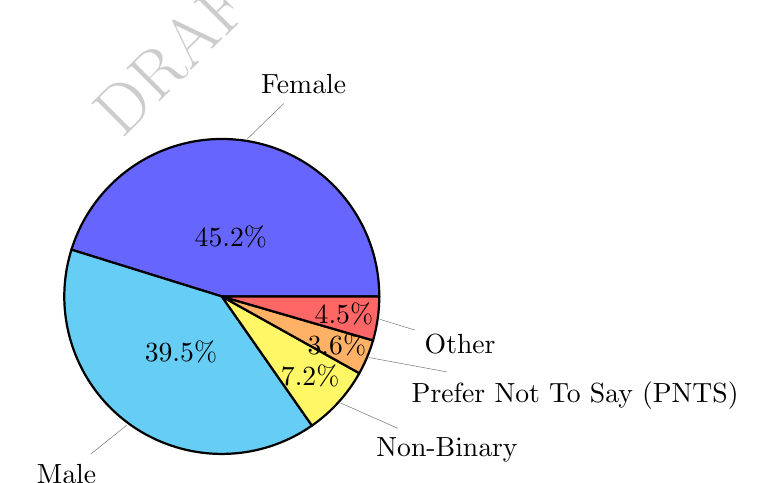
\begin{tikzpicture}
            \pie[text=pin, radius=2]{45.2/Female,
            39.5/Male,
            7.2/Non-Binary,
            3.6/Prefer Not To Say (PNTS),
            4.5/Other
            }
        \end{tikzpicture}
        \caption{What Is Your Identified Gender?}
    \end{minipage}\hfill
    \begin{minipage}{0.4\textwidth}
        \centering
        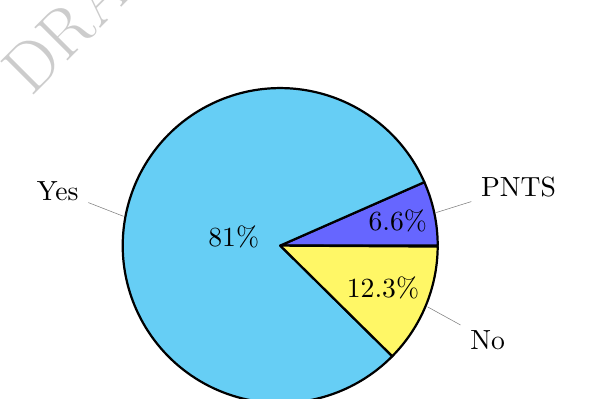
\begin{tikzpicture}
            \pie[text=pin, radius=2]{6.6/PNTS,
            81/Yes,
            12.3/No
            }
        \end{tikzpicture}
        \caption{Is Your Identified Gender Same as Birth Gender?}
    \end{minipage}
\end{figure}

\begin{figure}[H]
    \begin{minipage}{0.4\textwidth}
        \centering
        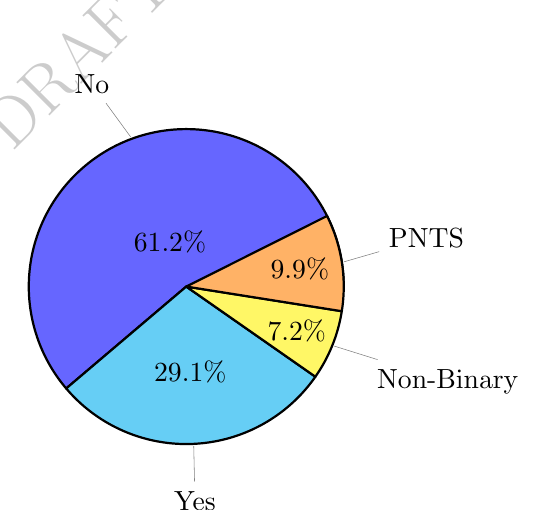
\begin{tikzpicture}
            \pie[text=pin, radius=2]{61.2/No,
            29.1/Yes,
            7.2/Non-Binary,
            9.9/PNTS
            }
        \end{tikzpicture}
        \caption{Do You Consider Yourself to be Neurodiverse?}
    \end{minipage}\hfill
    \begin{minipage}{0.4\textwidth}
        \centering
        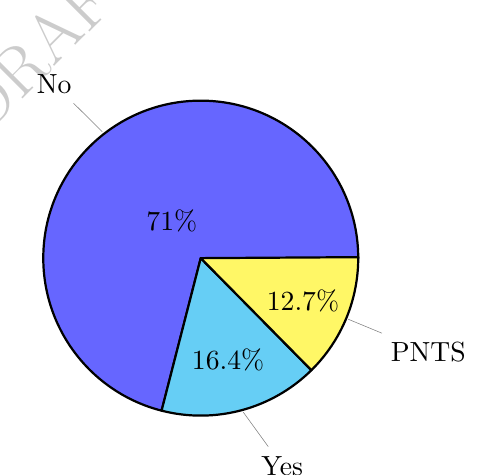
\begin{tikzpicture}
            \pie[text=pin, radius=2]{71/No,
            16.4/Yes,
            12.7/PNTS
            }
        \end{tikzpicture}
        \caption{Would you describe yourself as disadvantaged due to your mental health?}
    \end{minipage}
\end{figure}
\part{Supporting Events} % 5
    \chapter{Online Pre-Camp}
After seeing how Common Ground, Woodcraft Folk international camp held in 2022, ran their Pre-Camp sessions - it was decided to emulate this with a heavier emphasis on the online sessions. The online sessions took place from w/c 17 April to w/c 26 June with at least one session each week. Each session focused on a different component of the camp, ranging from a virtual site tour to a session where the attendees could meet the Site Services team.\\

Some teams found the online pre-camp sessions helpful, however on the whole - it was felt that they were stressful and time consuming. This point is further emphasised when reviewing the audience for each session. Most sessions only were attended by 2 to 4 attendees, with some gaining up to 20 additional views on YouTube after the fact. Some sessions, where recordings were actually taken, were published to the Woodcraft Folk YouTube channel.\\

No feedback was gathered beyond the core team, so we don't know the impact of Online Pre-Camp on the attendees.\\

On the whole, it would not be recommended to repeat Online Pre-Camp again in the same way in the future. However, taking learnings from this: it would be suggested that teams are given the opportunity to present an `update' which is recorded and published in some capacity, giving camp attendees information; with some teams still delivering a live session. The Food and Cafe \& Special Diets sessions were the best attended single-team sessions, it would be highly recommended to run similar sessions again. The General Q\&A \& broader sessions were also well attended, as would be expected - however many participants came along just to hear what was going on rather than ask specific questions, a testament to the team's excellent communications! The best-attended session was the Meet Your Village Evening, see below for further details around this. 

\section{How the Sessions Worked}
The majority of Online Pre-Camp sessions took a similar form:
\begin{itemize}
    \item Introductions to people hosting the session
    \item A short presentation, providing updates on that topic \& plugging future sessions
    \item Space for discussions and / or Q\&A
\end{itemize}

During each session, it was expected that notes were taken. The content of these notes was at the discretion of each session's facilitation team. For future sessions, it would be helpful to provide the facilitation team with a template they can insert their notes into rather than expect them to work out what to take notes on; thus ensuring what notes are returned to the coordinator after the session.\\

The sessions were promoted through our website. On the website, an events plugin enabled us to have a calendar which displayed upcoming events. An event was created for each Online Pre-Camp session, which gave us a space to link the Zoom Meeting from \& share any details about the session. A main Pre-Camp page also displayed information about Pre-Camp, should the movement want more information. Each week, a post was made to social media which detailed the upcoming sessions in that week - these were usually published in the first half of the week.\\

After each session, the event on the website would be updated to contain a link to the recording published to YouTube, any slides used, and any other relevant resources. 

\section{Sessions}
\begin{itemize}
    \item Welcome To Pre-Camp
    \item Virtual Site Tour
    \item Code of Conduct I (Day Scheduling and Leaving Site)
    \item Meet the Coordinator
    \item Booking Help
    \item Code of Conduct II (Respect, Clans \& Co-operation)
    \item Meet the Cafe / Allergy Teams
    \item Meet the Programme Team
    \item Meet the Food Team
    \item Meet the Site Services Team
    \item Meet Your Village Evening
    \item Code of Conduct III (Consent and Intoxicating Substances)
    \item Meet the Volunteer Support Team
    \item General Q\&A
\end{itemize}

\section{Meet Your Village Evening}
The biggest and most exciting session of the Online Pre-Camp series was by far the Meet Your Village Evening. This session was designed to announce the village allocations \& ensure village adults made contact with each other, a sort of first Village Meeting.\\ 

The session was regarded as a success - with all-bar-two groups booked present at the session, and some villages felt that their conversations had been so productive during the evening that they didn't require further meetings. From a coordination perspective, it was reassuring to know that key village adults had at least agreed on roles.
A follow up email was sent a few days after the evening, re-introducing those who had been at the session and introducing those who hadn't made it. This also shared links to the relevant forms which volunteers would need to fill in to say that they were taking on a role in the village or to request access to the Booking System. 

\subsection{Running Order}
Participants were given an overview of how villages would work and what would happen at camp. We also reinforced the aim of bringing everyone together and that this is our first Venturer Camp since before the pandemic. After a brief introduction and look at the map we showed the participants which groups would be in which villages and where villages would be on the site.\\

We spent some time talking about feeding central volunteers and explained which volunteers would be allocated where.\\

We then broke off into breakout rooms for each village, with a facilitator in each
\begin{enumerate}
    \item Introductions (names, pronouns, group \& role in group, all time favourite camp meal)
    \item Talk about equipment and who was supplying this 
    \item A space for the central volunteers to make themselves known
    \item Village Roles
    \begin{itemize}
        \item We said we needed names for: village coordinator, village KP (preferable more than one per village), Safeguarding lead, First Aid lead. Names don't have to be given tonight but note down ideas from people of who we could chase
        \item Optional extras (don't need names or need to dwell on this tonight): lost property keeper, KE/G (depends on where you're from), Fire, Programme, birthdays
    \end{itemize}
\end{enumerate}

We shared the form for village roles and said that these needed to be filled in as soon as possible. \\

Jeni, one of the people who ran this session, said it was Incredibly successful. We only had 2 districts coming to camp not turn up or send apologies
We need to have this session scheduled and in people's diaries as early as possible as it's really useful but more so if more people are there

    \chapter{On-Site Pre-Camp}
On-Site Pre-Camp was held at Biblins on the weekend of Friday 30 June - Sunday 2nd July. Not many members of the Core Team attended the event, in part due to dates and in part due to travel times. No leaders from delegations attended, despite being invited. We believe this to be due to the fact that many people in Woodcraft know Biblins well and wouldn't want to make the trek down there just to be told the same things they could find out online.\\

The dates were chosen to minimise exam clashes, which given the young nature of the Coordination team was for the best however it left us with very little time to do tasks and pick up actions after the event. This, whilst okay for some team members, left others with many actions to complete and little time to do them well in. The late date choice impacted other people not on the direct coordination team, for example getting the camp map designed.\\

There had been some discussion in the weeks leading up to pre-camp about if the event should go ahead or not, ultimately it did go ahead however some people felt the go or no-go decision needed to be made sooner as it resulted in confusion for some. It was also noted by attendees of the weekend that there wasn't an obvious booking contact for the weekend in the event that someone needed to cancel / amend their booking - while this did stop someone from cancelling their booking, it should be considered in the future. Furthermore, attendees who were in the central organising team but weren't core team didn't get any advanced information due to the Discord Structure. This is an oversight on the camp coordinators part, and the issues were rectified as soon as possible. \\

The agenda for the weekend was designed with fluidity and a chance for teams to take the time to do what they needed to do in mind. This resulted in a good balance of time where all the people present on site were taking part in site-wide activities and taking time to do what they needed to do in small groups (there were a series of bonus tasks completed throughout the weekend).\\

The pivotal moment during Pre-Camp was deciding the layout of the central area. Having this discussion on site enabled a participative \& cooperative approach where the majority of the relevant teams were able to contribute. Not having anyone with direct oversight of programme made this process slightly more complicated as it meant the people on site were relying on data in a number of spreadsheets to be up-to-date and from conversations had between team members to be able to decide placement for structures. Ultimately, this worked out fine - however it should be noted that when doing site layout, it's advisable to have members from the programme team present to determine marquee layout. \\

Another especially useful session was around teams sharing updates. This is something the coordinator had struggled to get teams to do in the leadup to this so having teams all in one place presented the perfect opportunity to share updates. Updates were varied, with some teams being basically ready for camp tomorrow and others still having lots of work - the Pre-Camp weekend displaying this to them and them then being able to get on with it.\\

The final major session of the weekend was Open Space. This time was utilised by some teams for them to have a team meeting where they could determine an actionable plan to take forward and complete; other teams did some maintenance at Biblins; and the remaining people took an inventory of the ex-Common Ground equipment and the ex-Crampton St. Office rooms within the Bunkhouse. In feedback from the weekend - some people found the inventorying to be a waste of time, however others thought it was invaluable as we now fully understood the equipment stored at Biblins, should we need to use any in the event of an emergency.\\

Jack Brown, working week \& takedown coordinator, led a session on what is happening during Working Week and Takedown - which was a very valuable use of time. Having this as the last session of the day proved very beneficial as we were able to use knowledge gained and decisions made earlier in the day to feed into this conversation, making it more productive.\\

Finding a KP for the weekend proved challenging. We were unable to source an external volunteer, which resulted in Noemi and Sabrina (ESC Volunteers based at Biblins) being tasked with KPing for us. They were supported by Lauren Karstadt with menu planning and ordering of food.\\

Throughout the weekend, the people on site at pre-camp were `left to it' with the food, after Noemi and Sabrina dropped it off for us on the Friday night. This was not how it had been sold to us, which caused some confusion. However we were able to make do given the number of competent Woodcrafters present! It was also noted during the evaluation that some of the specialist diets' food wasn't quite right - notably the Gluten Free options. \\

A good suggestion came out of the evaluation whereby for future events like this at Biblins, a member of the team should be encouraged to warden as this would then mean we have relative-unrestricted access to the Warden's Cabin with its electricity and WiFi! We were able to make do sitting on the balcony or on the grassy bank however had the weather been worse - we would've struggled. \\

It was felt that whilst the weekend on site proved extremely useful, it would be also extremely useful to have the entire team together. It was suggested that two in-person meetings could be held in the year of the event, one of them being in an easy-to-access meeting room in a city and the other being a site visit. From the coordinators perspective, this would be much more valuable as only having half the team present was a very difficult experience given the time pressure placed on us to pull off Venturer Camp in a year. 

    \chapter{Roadshow}
The Roadshow for Venturer Camp 2023 was a series of sessions facilitated by various members of the core team at regional events around the country in late 2022 and early 2023. These sessions aimed to spread the word of what was happening, gather potential participant's thoughts on the programme and answer leaders' questions.\\

It was decided to run these sessions as they had been done for previous camps, with greater success than ours however. Each of the different sessions went differently to each other, with some being great successes and others being less successful.\\

After some conversations, it was decided that it would be best to `piggyback' off of other events in the Woodcraft Folk calendar, rather than run our own events - due to the administrative \& financial impacts of running our own events. A session plan was devised by Woodcraft Folk's Chief Executive, which was designed with a number of sub-sessions in mind, so each Roadshow could be tailored to the audience, and time requirements.\\

The first roadshow was held in Scotland at their Scottish Gathering. This was a successful roadshow, probably due to the cohesive nature of the Scottish Nation in Woodcraft, and how core their Gathering is to their operations. This resulted in a large turnout of both young people and volunteers. The young people also re-wrote lyrics to a song which featured as part of an advert in the Venturer Camp news!\\

The roadshow then travelled to the Eastern Region for their first ever Eastern Region Venturers Fun day. This was facilitated by leaders based in the Eastern Region who were also on the Core Team. This was a successful event, mostly due to the fact that the target audience were present and the fact that the coordination team were experienced leaders who were able to take a session plan and engage young people \& adults in it.\\

The next stop for the Roadshow was the London Regional Gathering. This being a large event naturally meant that the Venturer Camp roadshow would be a smaller component than it was at either of its previous stops. Again, this was a successful event - gathering thoughts on programme activities from the young people in attendance and answering leaders' questions.\\

The Roadshow continued its journey south in the country to the South East Regional Gathering. This event was the least successful roadshow where any content was actually delivered. The event wasn't successful, due to the low number of attendees as well as the poor communications around the SE Gathering \& Venturer Camp roadshow. The low number of attendees, who were mostly adults, meant that the sessions designed to get participants talking had to be adapted and run as sessions for the leaders, still hoping to gather useful information. \\

The final stop for the Roadshow was supposed to be the biggest, as it was being planned to run as its own event. The event planning had all gone well, and we had agreed facilitators to run the event. We had planned to use a Youth Hostel Meeting Room in Manchester, as Woodcraft Folk has an agreement whereby they can access these facilities for free. A booking form had been created and circulated to Venturer Leaders through social media and our website. Unfortunately no one had booked. A decision was taken within the Woodcraft Folk Senior Leadership Team to cancel this event. This decision was communicated to the venue however not to any of the Volunteers working on the project. This resulted in the sessions facilitator finding out the session had been cancelled on arrival at the venue. This communication failure demoralised the team and soured the end of what, until this point, had been a successful roadshow.\\

The division of Roadshows around the country felt alright for a Venturer Camp sized camp. For a larger camp, it may be more beneficial to target all the functional regions \& hold general open access sessions, depending on what you wish to gain from them. Holding a roadshow virtually was also discussed but never happened due to time constraints, this could be a valuable opportunity to take. Piggy-backing off other events worked well, as our plans fit this well. It is suggested to repeat this. Generally the Roadshows were well received, with young people and volunteers alike getting excited about Venturer Camp 2023!

    \chapter{Working Week}
Working Week for Venturer camp was scheduled to begin on Wednesday 2 August, and run until midday on Saturday 5 August, when we allowed campers onto the site. During On-Site pre-Camp, the Camp Coordinator and Working Week coordinator decided that they would arrive on site on Sunday 30 July. \\

For the duration of Working Week and Pre Working Week, we were camping \& eating with Lewisham \& Greenwich, who were having their district summer camp on Pitches 6 \& 7. This was hugely beneficial to the Venturer Camp team as we were able to be fed and have shelter, without having to deal with it ourselves. However, from a KP's perspective: the Venturer Camp team was a nightmare to cater for. The KP has recommended not to do it in this way again, and that a separate KP should be sought for Working Week due to conflicting requirements of District Camp and Working Week. Members of the Working Week team were strongly encouraged to get involved with the meal preparation and clean up, to aid the Lewisham \& Greenwich team. The KP gave us a requirement of numbers for each meal, then it was up to the Venturer Camp team to find the people to fill this.\\

Having Lewisham \& Greenwich on site for the duration of Working Week also meant that we had access to the Luton Van which they had hired to transport their equipment. This proved extremely valuable as we were able to move equipment around the site with ease. It's helpful to have a few people confident to drive the van on-site as the requirement of this being on one or two people makes it more of a complex operation to move the van with needing to have the right people in the right places. \\

The pre Working Week days were used to organise and extricate equipment from the Bunkhouse storage rooms. It was decided that these days were needed after reviewing the relatively unorganised mound of equipment during on-site pre-camp. These days were instrumental in the success of Working Week, as there wasn't lots of time wasted on the first official day pulling tent poles out of a tiny room where only a few people could fit at once.\\

\begin{figure}[ht]
    \centering
    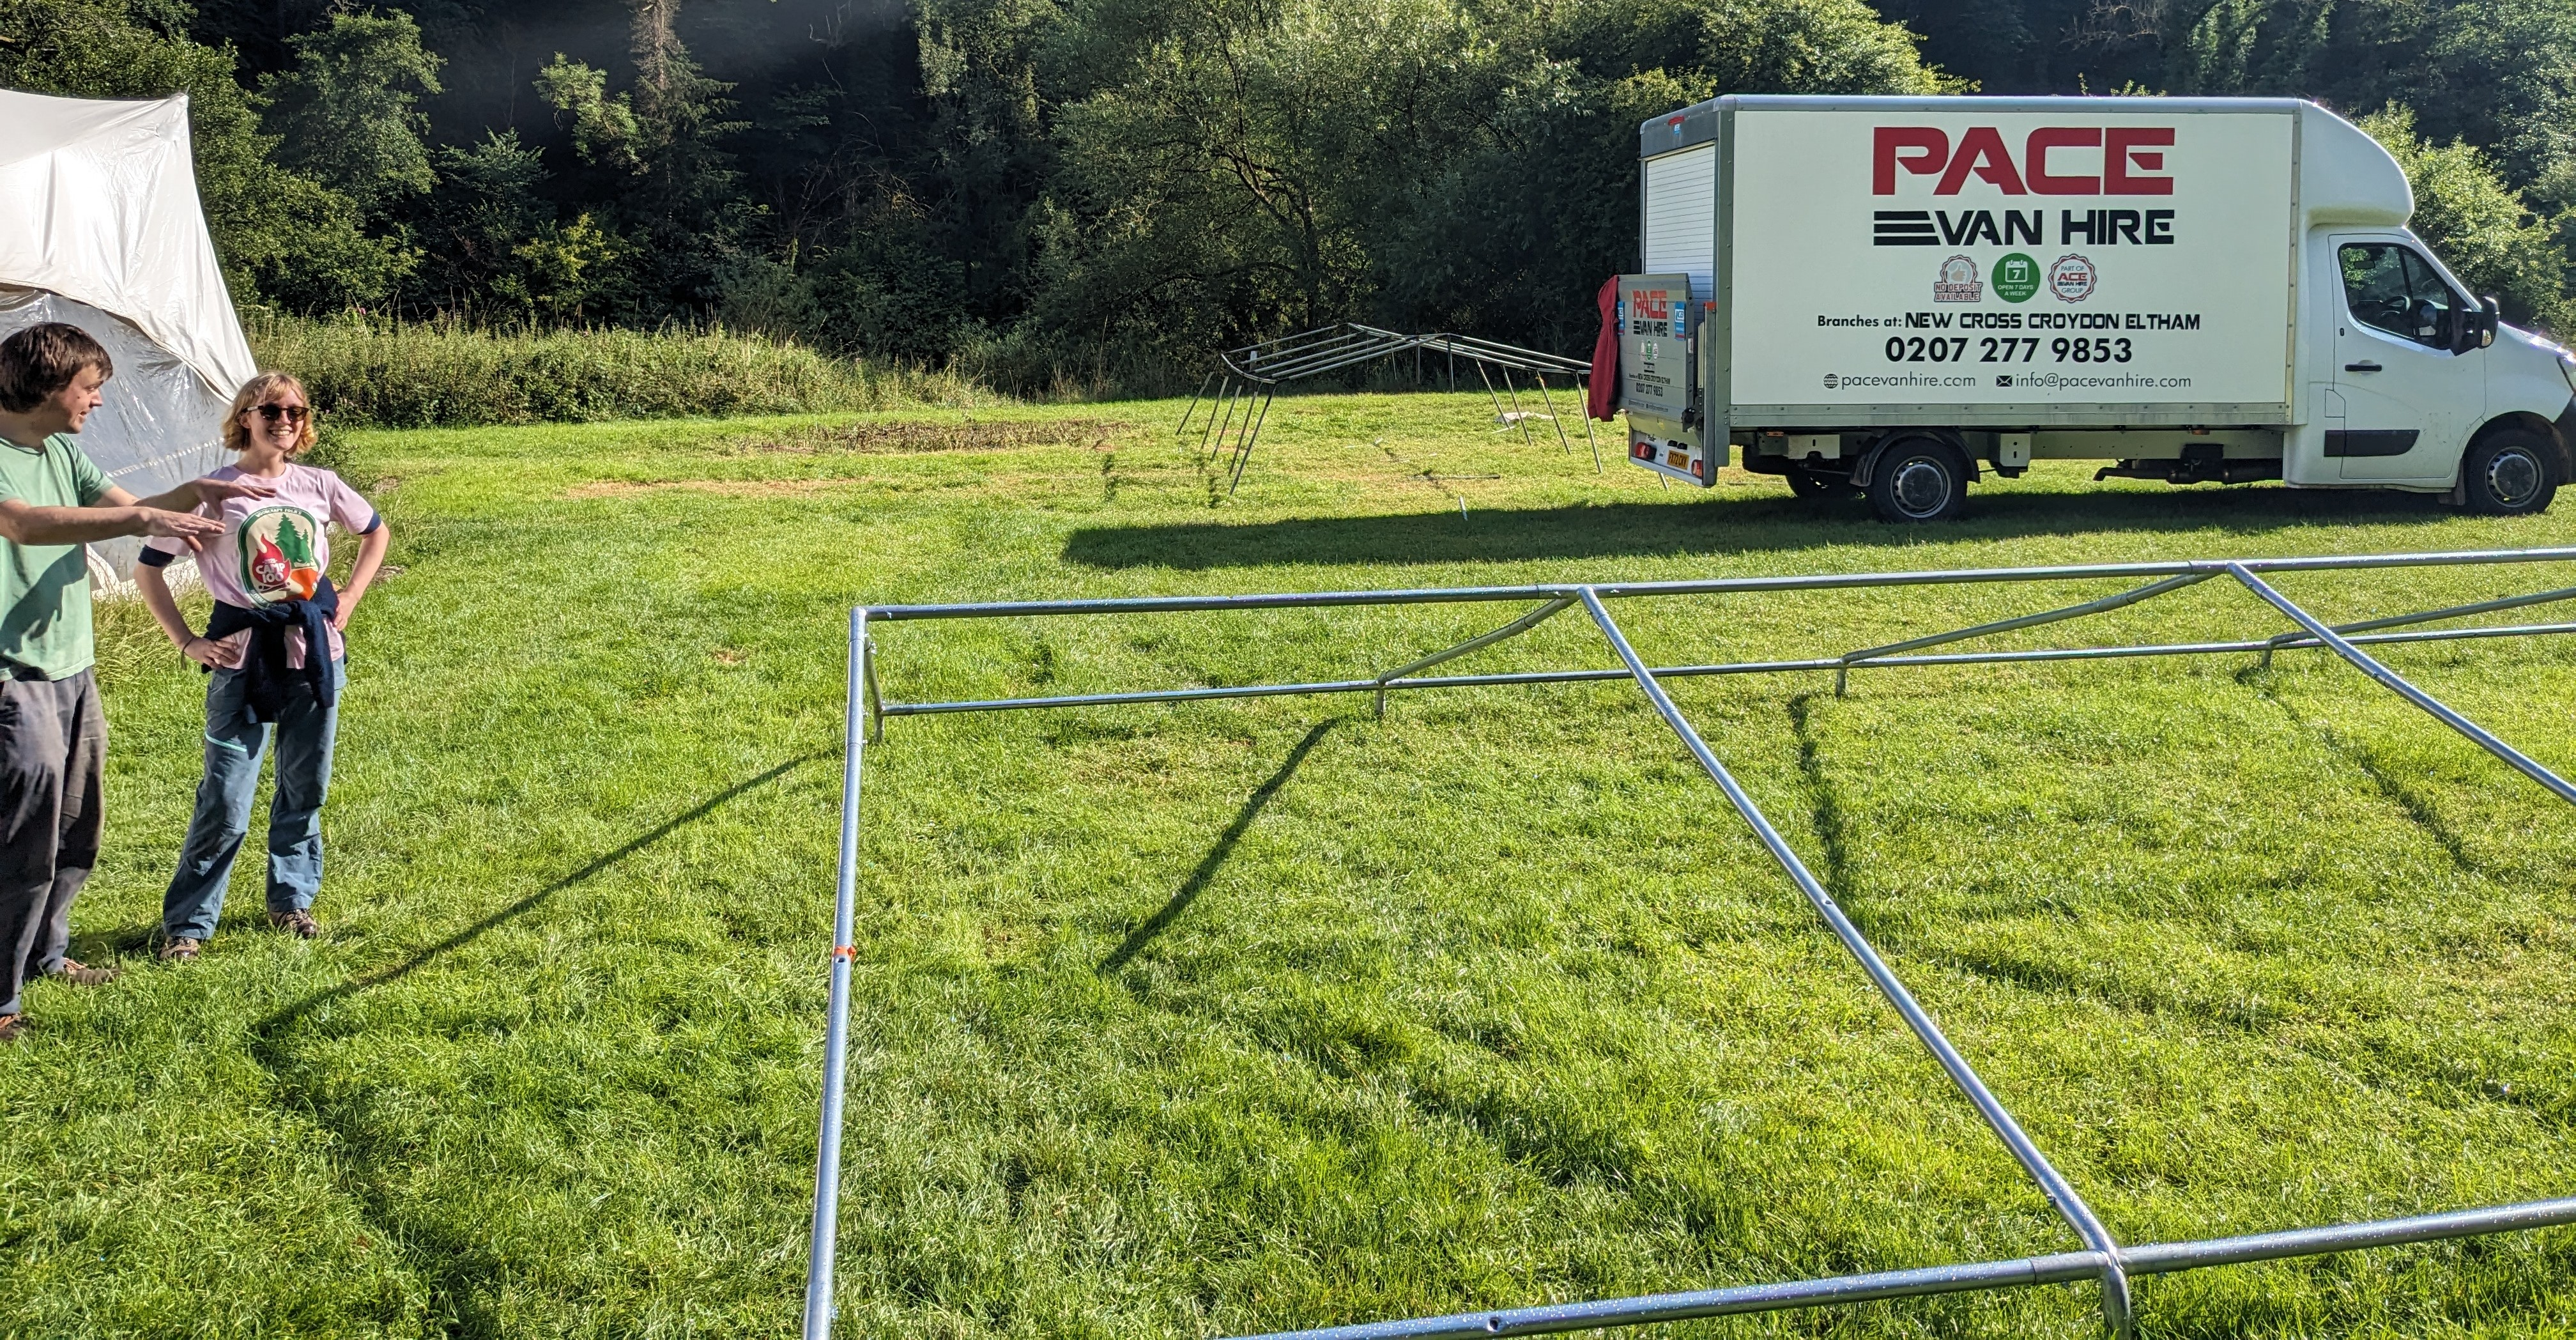
\includegraphics[width=0.8\textwidth]{assets/c100-coords-survey-5x10m-marquee.jpg}
    \caption{Camp100 coordinators survey one of the surviving 5x10m marquees as it's put up (\textit{TB})}
\end{figure}

On Tuesday 1 August, the Concordia team arrived to site. They spent the afternoon getting to know each other and the site with the ESC volunteers; then from morning on Wednesday 2 August - they got stuck in with the Working Week tasks. Altogether, we had 42 people book for some of Working Week, with 27 of these being on site from 2 August. This felt like the right number, however some additional people will always be useful! We managed to get all the required tasks done, however some of the administration was a bit of a squeeze towards the end. \\

As more people arrived for Working Week, they were keen to camp where they would be for the duration of the camp, rather than pitching on Pitch 6 for two nights then having to move. It was agreed that where no further groups were scheduled to be on the pitches, then Working Week attendees could camp where their village would be, this worked fine for the most part. \\

Having a dedicated coordinator for Working Week is extremely important. This is someone who works closely with the Coordinator to understand exactly what tasks need to be done and can lead the operational aspect of getting the site configured - leaving the Coordinator to deal with other, more complex problems. We were fortunate, in that there weren't many other problems - leaving the Coordinator to support with the site setup. A vague plan was devised ahead of time, building on discussions had at on-site pre-camp. This was useful and allowed for the Coordinator \& Working Week Coordinator to allocate tasks, especially surrounding people setting up their spaces on camp.\\

Each morning, a daily briefing was held over Breakfast - which enabled tasks for the day to be divided up \& people to share where they might need additional support throughout the day, or plan use of resources such as the van. Throughout the day, the Coordinator and Working Week Coordinator kept up to date with different teams - ensuring everyone was able to get on with their tasks. Walkie Talkies were used for communication, which is vital. It's imperative that these arrive to site fully charged and ready to go as waiting around for them to be charged wastes time.\\

\begin{figure}[ht]
    \centering
    \includegraphics[width=0.8\textwidth]{assets/working-week-breifing.jpg}
    \caption{Working Week Crew (\textit{TB})}
\end{figure}

Generally speaking, the right people were on site for Working Week. It would have been useful to have some more representatives from each centre present to ensure they were set up how they wanted it to be, however the Programme coordinator was able to fill in this gap. It proved very helpful to have a number of people who were able to support the large tasks, such as the Solar Array installation where a few key individuals were the masterminds behind it. Having additional people enabled the masterminds to conduct rather than do - preserving their energy for the camp itself!\\

During the week, large pieces of infrastructure got delivered to site. Much of this had been arranged by one person, with only them knowing the details of it or these details being stashed in a Google Drive folder somewhere. It would be useful for future events, for this information to be collated into the Working Week timetable so that we are able to easily allocate where the Porta-Loos are being placed or work out how big of a space we need to leave for the Main Marquee!\\

During the week, the Coordination \& Event Administration team worked closely with the Biblins site staff, forming relationships which proved extremely valuable for the camp.\\

Towards the end of the week, there were still a number of large groups on site who were scheduled to leave early on 5 August, the first day of camp. It would be beneficial to ensure that the site is booked for at least one day either side of the event itself as having the groups around made some things more complex, such as access to pitches. Generally speaking, other than one incident, the groups who were present on site during Pre Working Week \& Working Week itself were fine with us and didn't mind us being there. The incident was in relation to a group camping at the Eastern end of the site not wanting people driving past their pitch to access the canoe turning circle, which was required to turn the van around. 

    \chapter{Takedown}

Takedown formally started on the afternoon of Saturday 12 August, after the main camp had concluded \& attendees left. Due to site restrictions, we had instructed all attendees to be off site by midday as there were a number of other groups scheduled to be camping at Biblins that night. Takedown was scheduled to run until Wednesday 16 August, and the Burrow had been booked as such - however due to a desire to get away as quickly as possible, Takedown formally concluded at around lunchtime on Monday 14 August. Takedown was coordinated by Jack Brown, who is also one of the coordinators of Woodcraft Folk's next big camps. Having a dedicated Takedown Coordinator proved extremely helpful as they were able to take the lead on planning when equipment should be taken down and manage the storage of it, ensuring it was stored in a safe way for the 2025 camp.\\

On paper, it would seem that we had a good number of people booked to come to Takedown, with 25 coming. This figure included the 12 Concordia volunteers, so in reality - we had about 13 people at Takedown. Some of these people were only able to stay for one day, which left a very small group of people doing takedown. This was extremely difficult, as many of these people had been to Working Week and held key (high stress) roles on camp, which lead to a number of delirious moments throughout Takedown. Ultimately, we made it work - however for larger events where there would be more to do, this would be too great a task for the people left behind. For future camps, it may be worth exploring asking a Venturer or DF group to stay behind and support with Takedown. \\

To make the takedown crew's lives easier \& due to inclement weather, a decision was taken to strike as much of the central area as possible on Friday 11 August. This, whilst leaving the last night to have a strange looking central area, proved extremely valuable as we were able to drop 4 of the 5-by-10 m marquees after the central program finished. Whilst the Camp Coordinator \& Takedown Coordinator did end up orchestrating the taking down, extra people were able to be involved in getting the marquees down, sharing the load of the takedown.\\

The main food depot tent was also able to be taken down earlier in the day on Friday 11 August. This was returned to New Barnet overnight in the Luton Van, a decision which left us without the van on site to use to move the smaller centre marquees after taking them down - however a smart decision nonetheless, as it saved the hire of another van just to collect the marquee after camp. One of the parents of a young person drove the van to New Barnet and back, after being added to the insurance by the hirer. We were able to use a minibus on site to move the marquees, enabling them to be moved to the bunkhouse with ease. \\

The Luton Van had been scheduled to return Ealing's equipment to Ealing on Saturday morning, then return Lewisham \& Greenwich equipment to south London on Sunday where it would stay and not return to site. This left the takedown team with a shortage of van for the majority of Saturday and Sunday - something which had been planned for and we made work, however was another complication. Due to the lack of a van, we had to work in the earlier mornings and later into the evenings to ensure that all the required movements of equipment were managed; this was accompanied by using a car to transport some of the smaller, lightweight equipment. Having a van available isn't the only piece of equipment which is vital for a successful takedown - you also need some basic tools and ladders available for striking marquees, as we had hung lights high in the Ex-Swindon spiky marquee which we needed to de-rig. We were able to find a ladder on site to use, fortunately. \\

Villages generally were very good about getting their equipment taken down and off site by the specified time. Some villages chose to strike their large infrastructure the night before, in part due to early departures of some groups and in part due to inclement weather scheduled for Saturday 12 August. Villages were also generally pretty good about not leaving their pitches messy, other than one village who left a large amount of rubbish on the site. This was dealt with by the site staff team, however it should be noted for future that doing a full litter pick of the site may take a lot of people, a lot of time. \\

Some of the villages also opted to take down their sleeping tents, with the aim of minimising what had to be dried out after a potentially damp morning on 12 August. The Coordinator had given permission for the young people to bivy in the main marquee on the night of 11 August on the understanding that an appropriate ratio of adults would also be in the marquee. At 1am when the central programme finished, a member of Woodcraft Folk SMT overturned this decision which frustrated many campers, souring what had been a positive experience for the most part. For future camps, it would be beneficial to publish guidance and a suggestion around this ahead of camp. \\

In the evening of Sunday 13 August, the team (including the Concordias) had a meal from a fish \& chip shop for dinner then went to the pub for a celebratory drink. It is a tradition within Woodcraft camps to go to a pub for a meal, however we were unable to book a table large enough for all of us. This was a lovely way to conclude the main part of Takedown and gave the team some downtime before the final rush of activity on Monday Morning before the last people left the site. \\

Throughout the takedown weekend, meals were served out of the Burrow Kitchenette, which could just about cope with the size of our group. Leftover food which hadn't been donated to the Foodbank had been taken to the burrow towards the end of camp, which was turned into a number of simple meals. An oversight had been made in relation to the special diets, where not enough equipment or a sanitary space was available to cook these meals in - which is unacceptable. This was rectified by a small number of individuals cooking \& eating from the Warden's Cabin, until we had to close it for cleaning.\\

For future Takedowns, it's suggested that the Vengabus needs to be played more. This may sound strange to people who didn't come to takedown - however for those who were there, we can all still hear it. On a serious note, having a loud speaker and some good music can really help with takedown and morale. 

\part{The Team} % 6
    \chapter{Team Structure}

\section{Core vs Wider Team}
When the Coordinator began recruiting for Volunteers to fill out the majority of the team, an idea was vaguely mapped out that a smaller group of people would form the `core team', with support from the `wider team'. Work to recruit volunteers did fill the majority of the core roles initially, with many volunteers who hadn't been involved in a large camp before being recruited. Very quickly, the concept of a `core' and `wider' team was blurred, with it only remaining in the Discord server - roles such as centre coordinators \& stewards weren't assigned `core' access.\\

From a coordinator's perspective, it would've been beneficial to keep this structure in place - with a more defined support structure, as this would have reduced some of the repeated conversations, which may have saved some time. Generally speaking, the volunteer teams felt this way too. Volunteers agreed that a structure including team leads and supporting volunteers makes sense, considering the division of responsibilities and roles; furthermore it allows for more effective decision making by the core team. 

\section{Teams}
Broadly speaking, the individuals who were part of the Venturer Camp 2023 team fit into one of the following teams:
\begin{itemize}
    \item Coordination \& Event Administration
    \item Site Services \& Production
    \item Food
    \item Finance
    \item Volunteer Support
    \item Programme
    \item Stewarding
    \item Communications
    \item Transport Logistics
    \item Merchandise
    \item Sustainability, Environment \& Decarbonisation
\end{itemize}
Each team was structured slightly differently, their evaluations in the subsequent chapters will detail this. \\

There were a number of individuals who worked across a number of teams, for example a number of volunteers were involved in the Solar Power system (under Site Services \& Production's jurisdiction), and the Sustainability, Environment \& Decarbositation team. Considerations should be given here as to who they report to, we managed for Venturer Camp as the team supported each other however in the future plus the volunteers are extremely experienced; however in the future, we need to be more considerate of cross-team working like this. 

\section{Team Unity}
Due to the accelerated time scale in which Venturer Camp 2023 was organised, the unity \& bonding of the team was not as strong as it had been in the past. This was felt throughout the core \& wider team. Unfortunately, due to time pressures - we were unable to take the time to get to know each other and build relationships which would help to make the camp even better.\\

It was generally felt that the lack of in-person meetings contributed to the isolation some members felt. The only in-person meeting offered was On-Site Pre-Camp which had extremely low attendance due to the difficulties of getting to Biblins. For those who did attend Pre-Camp, there was a greater feeling of unity 

\section{Volunteer Recruitment}
Volunteers were recruited for Venturer Camp 2023 through a number of mechanisms, the primary being word of mouth at Common Ground. Having an international camp where the idea of a Venturer Camp is conceived works really well as lots of awesome Woodcraft Folk members are in a field who can be gently persuaded to take on a role at the next camp.\\ 

Further recruitment was done off the successes of Common Ground, using social media and email to reach members, inviting them to join an open meeting which enabled them to ask questions before getting involved. This worked well and filled out many of the remaining spaces on the team.\\

Unfortunately, not all roles were able to be filled. This included some significant roles such as Communications and Administration. These roles were less critical to fill as for the first time with a Venturer Camp - we had a dedicated member of staff working on it who could fill the gap. However, due to shortcomings in other teams, the member of staff's time was filled very quickly. This led to the Coordinator taking on some Production, some Communications, some Administration and some Finance tasks in addition to the Coordination role itself. Some of these additional tasks were shorter term due to either late recruitment or peaks in work. Having additional team members who could be used to plug these gaps would be extremely useful. \\

As would be expected with a large Woodcraft camp, recruitment continues right up until the end of camp for volunteers to take on a variety of roles. These late recruited roles ranged from Wide Game volunteers to stewards. The carefully calculated late-leaving of recruitment works, however it should be noted that for roles with age restrictions, for example, stewarding - can result in having to turn some people away. We ran into the fortunate circumstance where too many under-18s applied during camp for a shift. This left us overstaffed with under-18s and not enough over-18s to pad out numbers with the restriction in place that anyone aged under-18 needs to be paired with an over-18 while stewarding. \\

Venturer Camp 2023 also began to develop a suite of Role Descriptions for key roles. This is something which Woodcraft SLT requested that we do, as managing expectations for Volunteering roles is critical. For future events, it would be suggested to set the dates for any compulsory attendance meetings in advance, and require people to be available to attend to be able to take on the role. \\

We ran into an issue with a volunteer taking on a local group role as well as a significant central role. Due to ensuring the young people had sufficient leadership capacity, we were unable to allow the volunteer to take on both roles. This resulted in one of the teams loosing a core volunteer with lots of experience \& knowledge of the site. For future events, it would be suggested that the expectation that core team members only take on that role is made clear.

\section{Volunteer Onboarding}
Venturer Camp had no real Volunteer Onboarding process. This is something which it would be recommended to explore for future camps.\\

It was found that through not having a volunteer onboarding process, beyond ``join our Discord server'', we ran into issues where team members' contact details weren't available and it wasn't always clear what people were signing up for, either to themselves or to members of other teams. It would have helped greatly to have a short Google Form which new team members are expected to complete that asks for their basic information (email address, telephone contact number, role, etc) as well as any access needs they have and sets out expectations for meeting attendance etc. From this form, relevant data would be passed to relevant people which would hopefully enable people to feel better supported in the team as well as having more ways to contact them. 

    \chapter{Working Together To Make Venturer Camp Happen}
\section{Meetings}
\subsection{Online Meetings}
Monthly online check-in meetings were for the majority of the year leading up to Venturer Camp itself. These meetings were designed to check the progress of each team, understand where they have gotten to and work out where they are going next; a way of building shared accountability for the project. It was felt that the meetings would've been more engaging if there had been substantial discussions built into them - rather than sharing completed work. \\

The date and time to hold these meetings varied, a decision taken to ensure that the maximum number of people could be present. Unfortunately, some members of the team didn't engage in many (if any) meetings which lead to them not knowing anyone before they got to camp. \\

It was generally felt across the volunteer team that the meetings would be better if there were more decision-making and bonding activities planned as part of the agenda. It was suggested to have fewer meetings, with each being longer and more meaningful. \\

The online meetings were useful from a Coordination perspective as they were a very good time to get updates from teams, ensuring that teams were making required progress. Meeting with team members seemed to be the most productive way to get updates out of people, as when discussing team progress on Discord - teams would rarely respond which is extremely difficult to gauge progress from. 

\subsection{In Person Meetings}
To save time and money, it was decided that the only in person meeting held for Venturer Camp 2023 would be On-Site Pre-Camp, this would also double as the site visit. Whilst this was a good decision in terms of saving volunteer expenses for in-person meetings, it was a bad decision in terms of team unity \& building relationships between team members.\\

Woodcraft Folk members got very good at using technology to support their engagement through the Covid Pandemic where that was the only option. However, there is very little which compares to having people in a room building relationships, sharing ideas and feeling the excitement from each other about this thing which we are all working towards. \\

It is generally felt across the volunteer team that at least one more in-person meeting would have been beneficial. It was suggested to use a Youth Hostel Association Meeting Room in a large city or convenient location for the members of the team, as Woodcraft has access to these for free, for a day meeting or to have another residential meeting. For either of these options, careful considerations need to be taken as to who gets travel expenses paid to come - and this needs to be made clear in advance of the meeting.\\

It was also suggested that the in-person meetings could `tak-onto' another residential meeting taking place. For example, a General Council or Venturer Committee meeting could run in parallel to a camp committee meeting. This would reduce the overall cost per head for venue hire as well as provide space and time for lots of un-scheduled conversations which are often the most productive.\\

A suggested timeline for the in-person meetings, for Venturer Camp 2023, is shown below:
\begin{itemize}
    \item Late 2022 / Early 2023 - kick off meeting in a YHA in a city
    \item Spring 2023 - Team suggested to join a working weekend at the site to get to know the site
    \item June 2023 - On-Site Pre-Camp on site with team meeting element
    \item August 2023 - Camp itself
\end{itemize}

\section{Communications}
\subsection{Discord}
It was decided early on during the project conceptualisation phase that Discord, a popular instant messaging platform which is similar to Slack or Microsoft Teams, would be used as the primary communication platform for members of the Coordination team. This decision was taken due to the high levels of flexibility with which the platform can be used, and the Coordinator's familiarity with it. A positive side effect was that teams would be given a space in which they could converse with each other, without having to deal with setting up WhatsApp groups if they chose to use it.\\

Opinions about using Discord varied. Some volunteers found Discord effective and user-friendly, particularly for keeping discussions organised (through using channels \& threads) and for facilitating quick responses. However, there were a number of challenges which need to be addressed before Woodcraft uses Discord again. Some team members found it difficult to use and there was a need for better instructions around how to use it \& what the different areas of it were for which was highlighted during the evaluation. It was also sometimes felt that the information was scattered throughout it - making it hard to track down a critical piece of information. \\

It was generally felt that having a category per team, with a few communal categories worked well. Each category had a number of channels, which teams could edit and manage as they so chose. It was suggested that precisely what channels were made available to teams should be explored further as for some users the number of channels available to them was overwhelming. Again, users felt the need for better education around the use of the platform. \\

When new people were added to the server, they landed in a channel which required them to send a message containing their name and role on camp. This was used to assign the team members to the right places within the server. The Coordinator managed administration for the server, with another volunteer also having Administrative access should it be required.\\

A bot (carl-bot) was used to provide some additional functionality, such as auto assigning roles and reaction roles. It was suggested to look into a bot which can also send an email to a mailing list when a message is posted in an announcements channel. This is due to the fact that people would miss critical announcements as a result of not having their notifications configured correctly. 
\subsection{Inter-Team Communications}
In the lead-up to camp itself, some teams needed to contact other teams for a variety of reasons. This proved more challenging to teams than it should have. Through the Discord server, team members were able to identify members of the team to contact - however they weren't always sure who from a team to contact. A suggestion was made to have a who's who document linked from the Discord server identifying who to contact about different things. \\

It was also suggested that core team members should be given access to other team's general conversation channels, on Discord, to improve communication between teams.\\

Once team members were able to gain contact with the right person - the inter-team communication experience was positive, as you would hope within Woodcraft volunteers! 

\subsection{Other Communication Methods}
Some teams found it easier to communicate using other platforms such as Email \& WhatsApp. They used these other platforms as they would be their platform of choice or to avoid using crowded Discord channels. \\

All staff members were formally communicated with through their Woodcraft Folk email addresses. Many staff members engaged in the Discord server where they were given access to everything so they could communicate with teams there. For future camps, it would be suggested to do this in the same way, as having staff members accessible over an instant messaging platform works well. However, guidance should be given to volunteers on appropriate communications to staff as to not overburden them.


\section{Google Workspace Use}
As Woodcraft Folk utilises the Google Workspace as its cloud based productivity suite and email solution, it made sense for us to also utilise it. As part of the domain registration in Autumn 2022, the domain was re-configured as part of the Woodcraft Folk Google Workspace. 
\subsection{Google Drive Folder}
A folder for Venturer Camp 2023 was created within the Events shared drive. All team members were given access to this folder and instructed to store all their files in this folder. They were also instructed not to store secure files or files with sensitive content in this folder.\\

Feedback regarding the use of the shared folder was mixed, some members of the team found it efficient while others had difficulties in locating files due to folder naming and save-location issues. Members of the team would've been appreciative of a clearer folder structure and a more user-friendly approach.\\

A sub-folder was created for each team, as well as supporting events. This also applied for teams where there weren't people taking on those roles which may have led to the confusion. \\

With the Venturer Camp folder existing within the Events shared drive, this meant that lots of people had access to the Venturer Camp folder just by having access to the Events drive, which had been assigned for a previous event. This is a potential GDPR risk, especially with no volunteers receiving adequate Data Protection training. Due to this, it would not be recommended to follow this file saving approach in the future; with the recommendation being that each individual event gets its own Shared Drive created. After the event has concluded, the files can be moved to the main Events shared drive, for archival purposes. 

\subsection{Email Addresses}
As already discussed, we made use of the Woodcraft Folk Google Workspace, which included access to Gmail. We decided to use an individual email address system, rather than sharing passwords. This involved each member of the core volunteer team having their own personal @venturercamp.org.uk email address, with these being assigned delegate access to the shared team inboxes (for example, info@venturercamp.org.uk). As people understood how the system worked, they got the hang of it. However, it took members of the team some time to appreciate how the system works.\\

With the way Google manages delegate access to inboxes, you are unable to add this as an account on a mobile device without knowing the password, for this reason - it would be recommended to further explore how to do email addresses. Perhaps rather than a single individual holding all the passwords for all the accounts and dealing with all the delegation, it would be useful for a member of each team to know the password but be expected to use delegate access for the most part. 

    \chapter{On Camp Working}
\section{Volunteer Support}
Volunteer Support came in the form of the Positive Energy Bubble (PEB). PEB was located in the Camp Koodoo (adjacent to pitch 1a at the far-western end of the site) Marquee. This raised a number of concerns due to its location, being a 5 to 10 minute walk from the central area, and its size (a large marquee). Some volunteers were unable to utilise PEB due to the distance to get there and the requirement to climb steps to enter the marquee. \\

It was suggested that PEB should be centrally located, with the potential of it being used as a social space for adult volunteers in the evening. Volunteers also requested clearer communications about PEB's purpose and goals, which would enhance its effectiveness. \\

Volunteer Support would also have benefitted from additional capacity. There was one main leader of Volunteer Support who also had brought young people with them. They were supported by a number of other volunteers who ran small workshops. The lead Volunteer Support volunteer remarked that the trek from their Village (Elysium, pitch 9) to the PEB tent proved the most useful part of their day as they could stop and talk to people. 

\subsection{Support From The Coordinator}
The overall level of support from the coordinator was varied, with some teams feeling well-supported while others had limited engagement. Teams suggested that a consistent and proactive approach to support is necessary. \\

The Coordinator \& Events Assistant had hoped to split the teams between them, being a point of contact for the teams questions, concerns or ranting. However, due to the amount of additional work the Coordinator \& Events Assistant absorbed, they were unable to do this. Unfortunately, there was little capacity to support teams.

\section{Time Off}
A major focus for Venturer Camp 2023 was to ensure that all volunteers, whether they be a group leader or the coordinator, got some time off. This goal was built from feedback from Common Ground where volunteers didn't find that they had any downtime, leading to a large amount of burnout and exhaustion at the end of the camp. While we didn't get it right, as we still had a situation where the majority of a single team had to walk away for an afternoon on the same day, we definitely did better.\\

Many of the central volunteers managed to take some time off, with the majority opting for a day off. This took some planning and in some cases - drafting in of additional resources to plug gaps. However, the collective feedback indicates that having dedicated days off is essential for volunteer's wellbeing. Days off should be planned in advance of camp, not decided ad hoc, to ensure that adequate cover can be planned. It may be beneficial for teams to over-recruit volunteers to ensure that they can all take a day off without over-burdening others in the team. \\

Many volunteers found that socialising in the evening was a good way to relax. Some volunteers went off-site to the local village, Symonds Yat, before returning to site and looking for somewhere to socialise. When planning the camp, it hadn't been taken into consideration about the lack of spaces where volunteers could socialise. This lead to a number of instances where we had to ask Volunteers to move on and find somewhere else as they were disturbing sleeping Venturers. For future events, where there is not an obvious volunteer socialisation space, one needs to be provided. This may be the main marquee after the evening programme has concluded, or it may be the Volunteer Support space. 

\section{Feeding The Central Team}
Due to incidents at previous large Woodcraft Folk camps where central team members not camping as part of the Central Village didn't get food saved for them at meal times, we were very keen to improve on this. This was especially the case, given that we were not having a Central Village and having all the central team members camping in standard villages.\\

As part of the village handbook, KPs were given a list of people who needed food to be held back for them. This list was compiled by the Coordinator, ensuring that only the essential people were on this list as we recognised the large ask on KPs. Broadly speaking, the KPs were happy to oblige with this, understanding the need for it. \\

For future events - consideration should be given to those with allergies and how this is handled in relation to saving food. We had an unfortunate incident where a village had not saved food for one member of the core team, who had an allergic reaction as a result of cross contamination in the kitchen. \\

A number of members of the central team found that they needed more snacks provided. There were a few teams who had access to snacks, however there were teams who did not.

\section{Meetings}
Due to a shortage of time and capacity on site to organise a meeting, there was not a team meeting. Nearly all teams commented that having something like this would have been really nice and a good way to share experiences and increase team unity. It would have also been a time where teams could check in with each other, to ensure they all had enough capacity to get through camp.

\section{Shopping Trips}
Many teams had to take numerous trips off site to purchase additional resources. Some of these trips are unavoidable due to difficulties with deliveries, such as food deliveries, however some would've been avoidable with some slightly better planning. We tried to order as much as possible from online suppliers during camp, however due to Biblins being so isolated, deliveries took a long time to arrive. \\

Throughout the camp, there were a number of ideas raised which could've saved the number of individual trips off site, however none of these came through. The primary idea which would be great to see replicated in the future, is a single person going off site to do all the shopping. 

    \chapter{Staff Support}
Woodcraft Folk's Events Assistant was able to devote the majority of her 14 weekly hours to Venturer Camp from November 2022 until December 2023. This time was used to book major infrastructure, do some of the event administration, communications and support the Production and Programme teams, among other things. This role is managed by the Programme Manager, who also contributed some time in the last few months leading up to the event and on site. \\

The CEO of Woodcraft Folk put lots of time into this event from its conception, supporting the Coordinator and the programme team, leading on risk management and safeguarding both in the run up and on site, as well as helping with other things.\\

On site the Events Assistant, Programme Manager and CEO took on coordinator shifts along with the Coordinator and occasionally other volunteers. The CEO took on the majority of the safeguarding shifts with support from one volunteer and also the Head of Memberships \& Programmes (and Woodcraft's Designated Safeguarding Lead) at the very end of camp. With more than one volunteer coordinator and a volunteer safeguarding officer this level of support on site would not be needed.\\

From early May until the camp, the membership team supported us by doing membership and DBS checks, chasing those without them and supporting these people to sort it. This saved the camp team a lot of time compared to Common Ground when the Camp Assistant (staff administrator job role) did much of this. \\

The Head of Resources helped us set up accounts with food suppliers, and the finance team helped us pay invoices and expense individuals. Woodcraft's Fundraiser (Individual \& Legacy Giving) raised £6000 from the Christmas Challenge and this enabled us to offer an access fund to people who couldn't afford the full camp fee.\\

This camp had a lot more staff support than Venturer Camps have done in the past, with the creation of the new Events Assistant role and also the accelerated timeline for planning the camp meaning the team needed more support. It's also thought that since the pandemic volunteering attitudes, knowledge and experience have changed quite a lot, making it harder to recruit people. Some level of staff support is essential, with the Events Assistant role aiding continuity of knowledge between events and support from the experts on finance, membership and safeguarding. Hopefully future camps will not need this level of support, with a longer planning timeline and more young people moving into volunteer roles with experience developed from this camp, Common Ground and Camp 100.

    \chapter{Concordia}
Woodcraft Folk worked with the company Concordia to recruit a team of international volunteers. This was the first time that Woodcraft has worked with Concordia and as such there were a number of teething difficulties.\\

A representative from Concordia visited the site in March 2023 to conduct a Health \& Safety audit. As part of this, the decision was made that the Burrow would act as a base for the Concordia team. This decision was not effectively communicated to the team at the time as until this point, it had been vaguely agreed that the core team would have access to the burrow as a place to sleep with better beds and a small kitchenette which the team could use to reheat food should they require this.\\

Concordia managed the recruitment of volunteers. While this saved time for the Venturer Camp team, it proved challenging to get this information out of Concordia. Specifically, their dietary requirements and any access needs were not communicated until after the standard booking deadline and one volunteer's information not being shared until days before the first members of the team were on site. In the end, we had nine volunteers, who all arrived in the country and were helpful with some tasks they were assigned. \\

In the lead up to the event, Woodcraft Folk's Programme Manager made repeated attempts to gain direct contact with the volunteers themselves however Concordia were reluctant to divulge the volunteers phone numbers. Ultimately, however, the Programme Manager was successful in gaining contact with the team. This allowed limited information to be shared with the volunteers. Unfortunately, this information came too late for many of the volunteers who had already packed and were unable to bring suitable clothing or prepare for their time at Venturer Camp. This led to a decreased spirit amongst the team and a general reluctance to do things.\\

Due to the lack of communication with the volunteer team in advance of the camp, no expectations were able to be set from Woodcrafts side. This led to a very harsh reality on the first night where we had to put the team up in tents rather than the burrow. Whilst the team did have suitable tents and sleeping mats provided from Biblins and the room of strategic requirement, a number of them did not bring suitable clothing for that night. The volunteer team also had the expectation that they would have more time off during the event. This led to lots of disappointment when they couldn't go off site to a Pub as they were needed to support other activities on site. \\

On-Site the two Centres ESC Volunteers were tasked with supporting the engagement of the Concordia volunteers. The two volunteers had training sessions with the Concordia staff team as well as the WCF Programmes Manager. Unfortunately, on site, the two ESC volunteers were not able to support the Concordia volunteers effectively which further led to low spirits within the international volunteers.\\

During Working Week, camp itself and takedown, the Concordia volunteers needed to be told exactly what to do and when. As this was their first experience of Woodcraft Folk and the way we camp, and for many of them - their first experience in a camp setting, they were unable to take initiative or move on to another task once what they were doing had been completed. This resulted in some confusion for them and frustration for the Woodcraft volunteers \& staff when the Concordia team wouldn't show up or they would not engage with changed plans, which unfortunately happened numerous times.\\

Due to an administrative error when reviewing the draft contract from Concordia within Woodcraft Folk, the Concordia volunteers were scheduled to arrive on Tuesday 1 August and depart on Monday 21 August. This error led to us having to put them in tents the first night they were on site. Luckily, we were able to provide this equipment for them, however the tents were not treated particularly well. Many of the doors were left open during the days following their use, when it rained heavily, hence we couldn't take them down. When the tents were finally taken down, they were thrown in a heap rather than being packed back into their bags. These actions resulted in the exhausted Woodcraft volunteer takedown team needing to do extra work to clear up after the Concordia team.
The date the Concordia team was booked to depart was later than that originally advertised to the Coordination team of the camp. This resulted in some confusion amongst both the Woodcraft Volunteers and Concordia team. Ultimately, all the members of the Concordia team paid to change their flights / booked new flights to depart on either the 16 or 17 August. \\

The volunteers showed they had the independence to navigate trips to shops and pubs (neither of which are particularly close to site), but did not apply this to tasks on site and often did these things when they were meant to be on shift either at the time or early the next morning when they often didn't show up because they were still asleep.\\

We were very clear in all our communications about the camp (including the info packs we sent Concordia) that there would not be much signal or Wifi on site. However Concordia failed to pass this info on, and as a consequence we felt we had to share the wifi with the volunteers so they could keep in touch with friends and family. This meant they were often hanging around the cabin to use the wifi, making it slow for people needing it to make the camp happen/run the site, and bothering other volunteers/staff for the password when we had to change it so the staff on site could do their jobs. \\

The volunteers were very helpful when it came to putting up lots of 5x10m marquees in working week, and also some of them supported other jobs really well e.g helping the shuttle bus volunteers on arrivals and departures days, some stewarding shifts etc. However overall, it was more work for us to manage them and give them things to do, plus paying for their food and board, than the little work they did on site. This is partly due to lack of planning and understanding on our part, and partly due to Concordia not delivering what they said they would in terms of giving us and the participants the information we needed.\\

It would not be recommended to work with Concordia again for the reasons outlined above. Should Woodcraft Folk decide to work with them again, written assurances should need to be provided to the Camp Coordinator / Project Manager that the issues outlined above will be addressed and resolved to the satisfaction of Woodcraft Folk

\end{document}


%table template
\begin{table}[h]
    \centering
    {\RaggedRight
    \begin{tabular}{p{0.2\textwidth} p{0.2\textwidth} p{0.2\textwidth} p{0.3\textwidth}}
    \textbf{Name} & \textbf{Predecessor} & \textbf{Successor} & \textbf{Examples}\\
    \hline
    \hline
    Linear & unique & unique & stack, queue\\
    \hline
    Hierarchical & unique & many & family tree, management structure\\
    \hline
    Graph & many & many & railway map, social network\\
    \hline
    Set Structure & no & no & DSALG class\\
    \hline
    \end{tabular}
    } % end of rr     
    \caption{Classifications of Data Structures}
\end{table}